%%%%%%%%%%%%%%%%%%%%%%%%%%%%%%%%%%%%%%%%%%%%%%%%%%%%%%%%%%%%%%%%%%%%%%%%%%%%%%%%
% experiment.tex: Chapter describing the experiment
%%%%%%%%%%%%%%%%%%%%%%%%%%%%%%%%%%%%%%%%%%%%%%%%%%%%%%%%%%%%%%%%%%%%%%%%%%%%%%%%
\chapter{The CMS Experiment}
\label{experiment_chapter}
This chapter details the CMS experiment as well as the CERN accelerator, the Large Hadron Collider (LHC), which is used by CMS. Specific attention is paid to the components of CMS and the LHC most relevant to the \WR search.
The \LHC is the largest and highest-energy particle collider ever created.  It is a 27 kilometer circumference synchrotron accelerator with two beam pipes each designed to carry approximately 2700 bunches of protons which can be brought into collision at four interaction points around the ring. The four experiments around the ring, clockwise looking down, are \ALICE, \CMS, \LHCb, and \ATLAS.  It was first operated with \rootsseven, then \rootseight, and now \rootsthirteen.

\begin{figure}[!tp]
    \centering
    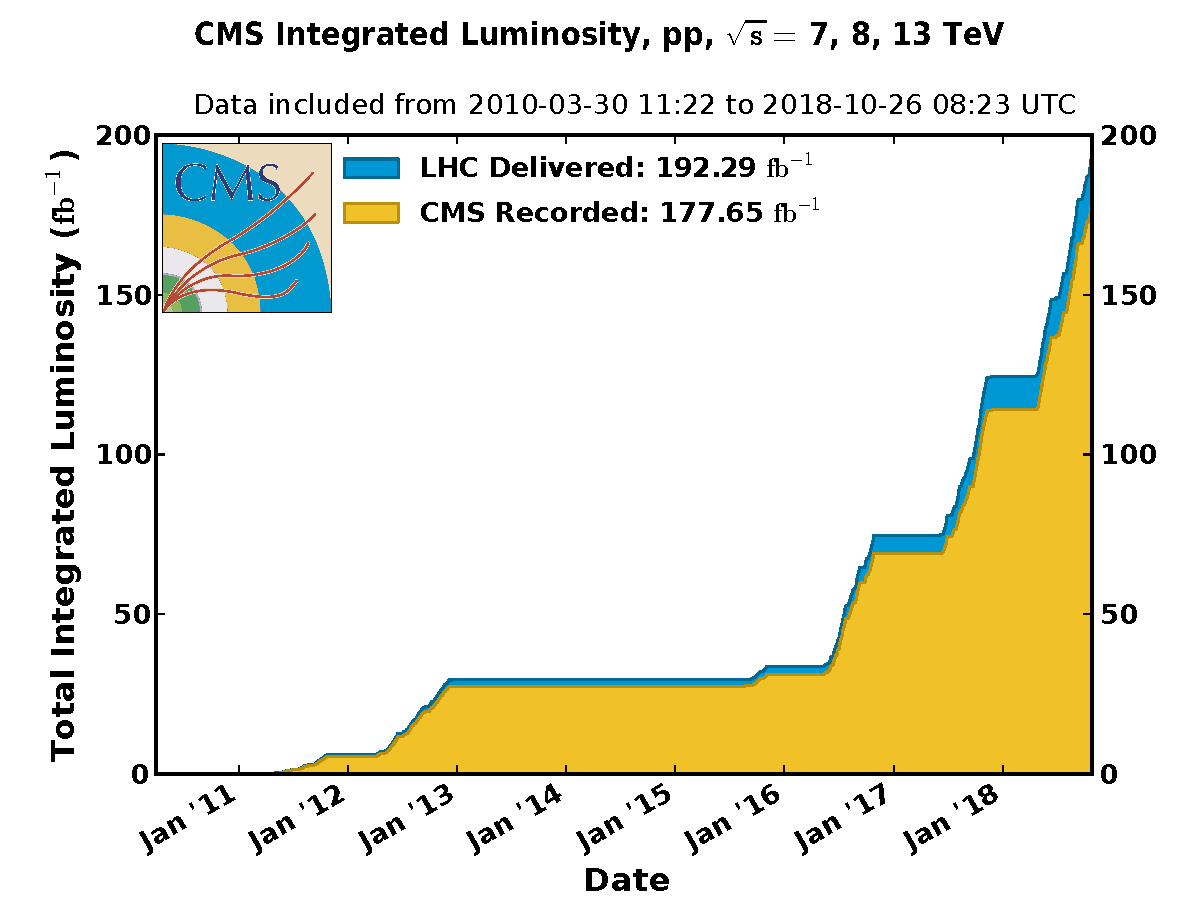
\includegraphics[width=\textwidth]{figures/int_lumi_allcumulative_pp.pdf}
    \caption[
        %short caption
        Multi-year delivered luminosity of the \LHC
    ]    
    {
        This graph shows the integrated luminosity of the \LHC over all the years of operation.  It can be seen that recent years have seen a dramatic increase in instantaneous luminosity, with the last year, 2018, contributing approximately one third of the total.
    }
    \label{fig:lhc_delv_lumi}

\end{figure}

\section{The Large Hadron Collider}
The \LHC was constructed outside Geneva, Switzerland.  It was first operated in the Fall of 2008, and after a magnetic failure, was repaired and recommenced operation in 2010. The \LHC is part of an accelerator system.  Each accelerator adds a portion of energy to the beam, progressively increasing to the LHC injection energy.  The start of the \LHC proton beam is a humble gas bottle of hydrogen gas.  From there, the gas is ionized and accelerated with a linear accelerator (LINAC 2) which accelerates protons directly into the Proton Synchrotron (PS).  The PS accelerates the protons to an energy of \SI{26}{\GeV} before injecting them into the Super Proton Synchrotron (SPS).  The SPS accelerates proton bunches up to \SI{450}{\GeV}.  Once proton bunches have reached this energy they can be accelerated into the \LHC. These bunches are then accelerated to \SI{6500}{\GeV}.  The \LHC was originally designed for operation at up to \rootsfourteen but has not done so yet. In the last data taking period, which concerns this analysis, the \LHC ran at \rootsthirteen.

Protons are accelerated in each of the synchrotrons with radio-frequency (RF) cavities.  The RF cavities fill the beam path with standing electro-magnetic waves. Protons passing through the standing waves are accelerated and kept in bunches. Slow (and behind) protons are accelerated more than faster (and leading) protons in each bunch. This ensures that each bunch of protons is well-formed in momentum and physical space. At the LHC, there are 8 RF cavities for each beam and they are operated at \SI{400}{MHz}. Bunches collide at intervals of \SI{25}{ns}.  This is part of the design of the RF cavities, as a bunch is accelerated every 10 cycles of the radio frequency. This gives a maximum number of bunches at the LHC of roughly 3600. Each step in the synchrotron acceleration chain requires additional space so that injection (and dumping) magnets can be brought to full energy in between bunches. This gives an actual total of 2808 bunches.

While the \LHC holds the record for the highest center of mass energy per nucleon of any hadron collider built to date, allowing it to probe previously unreached mass regions, it is also the most luminous hadron collider.  The record instantaneous luminosity and a high-duty cycle has allowed the \CMS experiment to record an unprecedented number of collisions.  The luminosity, shown in equation \ref{eq:lumieq}, is proportional to a number of factors

\begin{equation}
    \luminosity = \frac{fnN^{2}\gamma}{4\pi\epsilon_{n}\betastar}F
    \label{eq:lumieq}
\end{equation}

Orbital frequency, \ensuremath{f}, is the frequency a given bunch interacts, \ensuremath{n} is the number of bunches of protons in each beam, \ensuremath{N} is the number of protons in each bunch, \ensuremath{\gamma} is the Lorentz boost of the protons, \ensuremath{\epsilon_{n}} is the beam emittance, \betastar is the beta function, and \ensuremath{F} is based on the shape of the beam crossing.  Emittance and the beta function describe the focusing of the beams as they cross.  Multiplying them together gives the square of the cross-section area of the beams at the crossing point.  At the \LHC the number of protons per bunch, the number of bunches and the beam cross-section at collision can be changed.  It can be seen from \ref{eq:lumieq} how these parameters affect the luminosity.  Increasing the number of bunches and the protons per bunch increase luminosity.  Likewise, focusing the beams to a small cross-section increases luminosity.  Each of these variables have their limits and challenges associated with changing them.  The total number of bunches the \LHC can hold is predefined by the frequency of the RF cavities as well as the need for injection and ejection of the beams in the accelerator chain.  The number of protons per bunch, without changing the bunch size, or conversely keeping the number of protons per bunch the same and reducing bunch size, can be done but it is technically difficult.  Higher proton density bunches are more difficult to control and can become unstable.  Higher proton density in bunches also leads to an increase in additional proton interactions in a given crossing.  This poses a challenge to the detectors to sufficiently determine the properties of the interaction of interest and increases the rate of radiation damage in the detector.
The first year of operation saw \GLNTEN delivered luminosity at \rootsseven.  The accelerator continued operation at this energy for 2011 delivering \GLNELEVEN.  In 2012 the energy increased to \rootseight and \GLNTWELVE were delivered.  After a longer shutdown for three years and significant upgrade work, the \LHC resumed operation at \rootsthirteen and ran for 2015, 2016, 2017, 2018.  A total of \GLNTOTALII was delivered over those four years. During Run II, 2015-2018, the \LHC was operated at its tightest bunch spacing of \SI{25}{ns}. The first year of Run II, 2015, was considered a commissioning year and collected significantly less data and is not considered in this analysis.  From 2016-2018 the \LHC continued to outperform itself, increasing the number of protons per bunch beyond design specifications and ultimately delivering \GLNTOTALII collisions.  Some of the relevant parameters for the three years covered in this analysis are summarized in \ref{tab:lhc_design_specs}.

\begin{table}[]
    \centering
    \begin{tabular}{|c|c|c|c|}
        \hline
        Parameters & 2016 & 2017 & 2018\\
        \hline
        Beam Energy & \SI{6.5}{TeV} & \SI{6.5}{TeV} & \SI{6.5}{TeV}\\
%        \betastar & \SI{IDK}{m} & \SI{IDK}{m} & \SI{30}{cm}\\
        Bunch Spacing & \SI{25}{ns}& \SI{25}{ns}& \SI{25}{ns}\\
        Number of Bunches & 2808 & 2808 & 2808 \\
 %       Protons per Bunch & & & \\
  %      Normalized Emittance at Start of Fill & & & \\
        Peak Luminosity Per Day & \SI{15.3}{Hz/nb}& \SI{20.7}{Hz/nb}& \SI{21.4}{Hz/nb}\\
        Mean Number of Events per Crossing & 27& 38& 37\\
        Delivered Integrated Luminosity & \GLNSIXTEEN& \GLNSEVENTEEN& \GLNEIGHTEEN\\
        \hline
    \end{tabular}
    \caption[LHC operating parameters]{Operation parameters of the LHC during Run II, 2016-2018.}
    \label{tab:lhc_design_specs}
\end{table}

\begin{figure}[!tp]
    \centering
    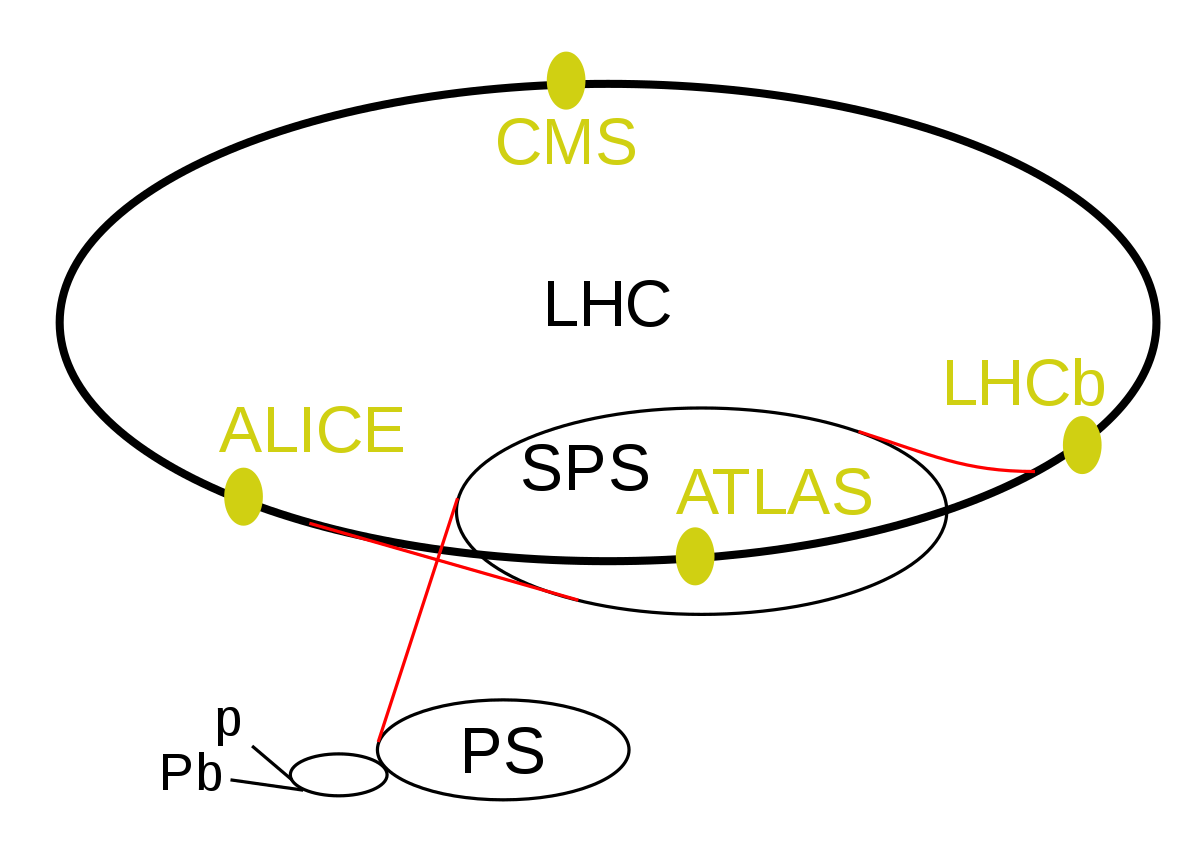
\includegraphics[width=\textwidth]{figures/1200px-LHC_svg.png}
    \caption[
        %Short caption for the list of figures
       LHC accelerator complex.
    ]{
        % Full caption shown below the image
        This diagram shows the accelerator complex feeding into the LHC.  Starting with a linear accelerator, the protons are accelerated into the Proton Synchrotron (PS) and then Super Proton Synchrotron (SPS) before injecting into the LHC. 
    }
    % A label so you can \ref{fig:my_fig}. It is arbitrary; neither the 'fig:'
    % nor the fact that it has the same name as the pdf are required.
    \label{fig:lhc_diag}
\end{figure}



\section{The Compact Muon Solenoid}
The Compact Muon Solenoid (\CMS) at CERN is one of the general purpose detectors at the \LHC and the one used for this analysis.  Each part of the detector is built around the previous moving outward from the interaction point in a cylindrical shape.  Through the long axis of \CMS runs a single beam-pipe containing both proton beams which are brought into collision in the very center. \CMS is designed to accept as many events as possible and with as much detail as possible.  It covers a large solid angle to allow for as many of the post-collision particles as possible to encounter an active part of the detector.  \CMS also has extremely fast electronic readout to allow it record events as often as possible and as accurately as possible.

The CMS detector has several major detector components, sub-detectors, as well as a very large solenoid magnet. A drawing a \CMS and its different components is shown in \cite{Sakuma_2014}. The support for these components is integrated as part of the magnet return yoke.  Starting at the interaction point and moving outward transversely, the CMS detector is made up of a silicon-tracker, an electromagnetic calorimeter (ECAL), a hadronic calorimeter (HCAL), the magnet, and then the muon chambers with an iron magnet return yoke interspersed.  Each of these parts will be discussed further shortly. Additionally the detector changes on the two ends of the cylinder, called endcaps, this is to account for the differing particle fluence at different collision angles.  

As the \CMS detector is discussed, it is first helpful to describe the coordinate system used.  This coordinate system is standard for hadron collider experiments.  The Cartesian coordinates are defined as follows: \ensuremath{x} points to the center of the collider, the \ensuremath{y} points up, and the \ensuremath{z} coordinate points in the counter-clockwise, looking down, direction along the beam.  This creates a right-handed coordinate system.  The origin of these coordinates lies at the center of collisions within the detector.  An angular coordinate system is generally used to better reflect the geometry of the particle collisions and the detector itself.  This coordinate system is defined with \ensuremath{\eta}, \ensuremath{\phi}.  Here, \ensuremath{\phi} is simply the azimuthal angle in the \ensuremath{x-y} plane and \ensuremath{\eta} is defined as pseudo-rapidity:
\begin{equation}
    \eta \equiv - \ln{
    \tan \left(\frac{\theta}{2}\right) }
    \label{eq:pseudorapidity}
\end{equation}
In this equation, \ensuremath{\theta} is the the polar angle along the \ensuremath{z} axis.

Pseudo-rapidity is used as a simpler alternative to particle rapidity defined with the particle momentum along the beam direction and its energy.
\begin{equation}
    Y \equiv \frac{1}{2} \ln{\left( \frac{E+p_z}{E-p_z} \right)}
    \label{eq:rapidity}
\end{equation}
When a particle is massless, the \ensuremath{Y} simplifies to \ensuremath{\eta}, which is a good approximation considering the energies of particles at the \LHC.

At \LHC energies, proton collisions actually involve the collision of individual components of the protons, quarks and gluons.  The momentum of these partons is not known during the collision.  The result is that each collision has a different amount of boost along the \ensuremath{z} axis.  
However, the rapidity of a particle does not change when the particle is boosted along the \ensuremath{z} axis.  As such, defining a coordinate system with \ensuremath{\eta} (which approximates \ensuremath{Y}) allows for post-collision particle directions to be discussed in a way roughly invariant of their initial momentum in the \ensuremath{z} direction.  Given the large inelastic cross-section at the \LHC, this also guarantees that any given sweep of \ensuremath{\Delta \eta} will have roughly the same particle fluence.

As a result of the unknown longitudinal momentum, a particle's momentum and energy is generally only considered in the transverse direction.  The transverse components are calculated from \ensuremath{\eta}.  The transverse momentum and energy of a particle is defined as
\begin{equation}
    p_T \equiv |p| / \cosh{\eta} 
    \label{eq:pT}
\end{equation}{}
\begin{equation}
    E_T \equiv E / \cosh{\eta} 
    \label{eq:Et}
\end{equation}{}

Energies and momenta determined from the detector can then be re-expressed independent of the particle's longitudinal boost. The \ensuremath{\eta} and \ensuremath{\phi} are also used in conjunction to calculate particle's separation independent of their longitudinal momentum as well.  This is defined as \ensuremath{\Delta R}
\begin{equation}
    \Delta R \equiv \sqrt{\Delta\eta^2 + \Delta\phi^2} 
    \label{eq:dR}
\end{equation}
\subsection{Particle Flow}
At \CMS every candidate particle is reconstructed using as many subdetectors as may contain information about the particle. A diagram of what this process looks like is shown in Fig.~\ref{fig:particle_flow_cms}.

\begin{figure}[!tp]
    \centering
    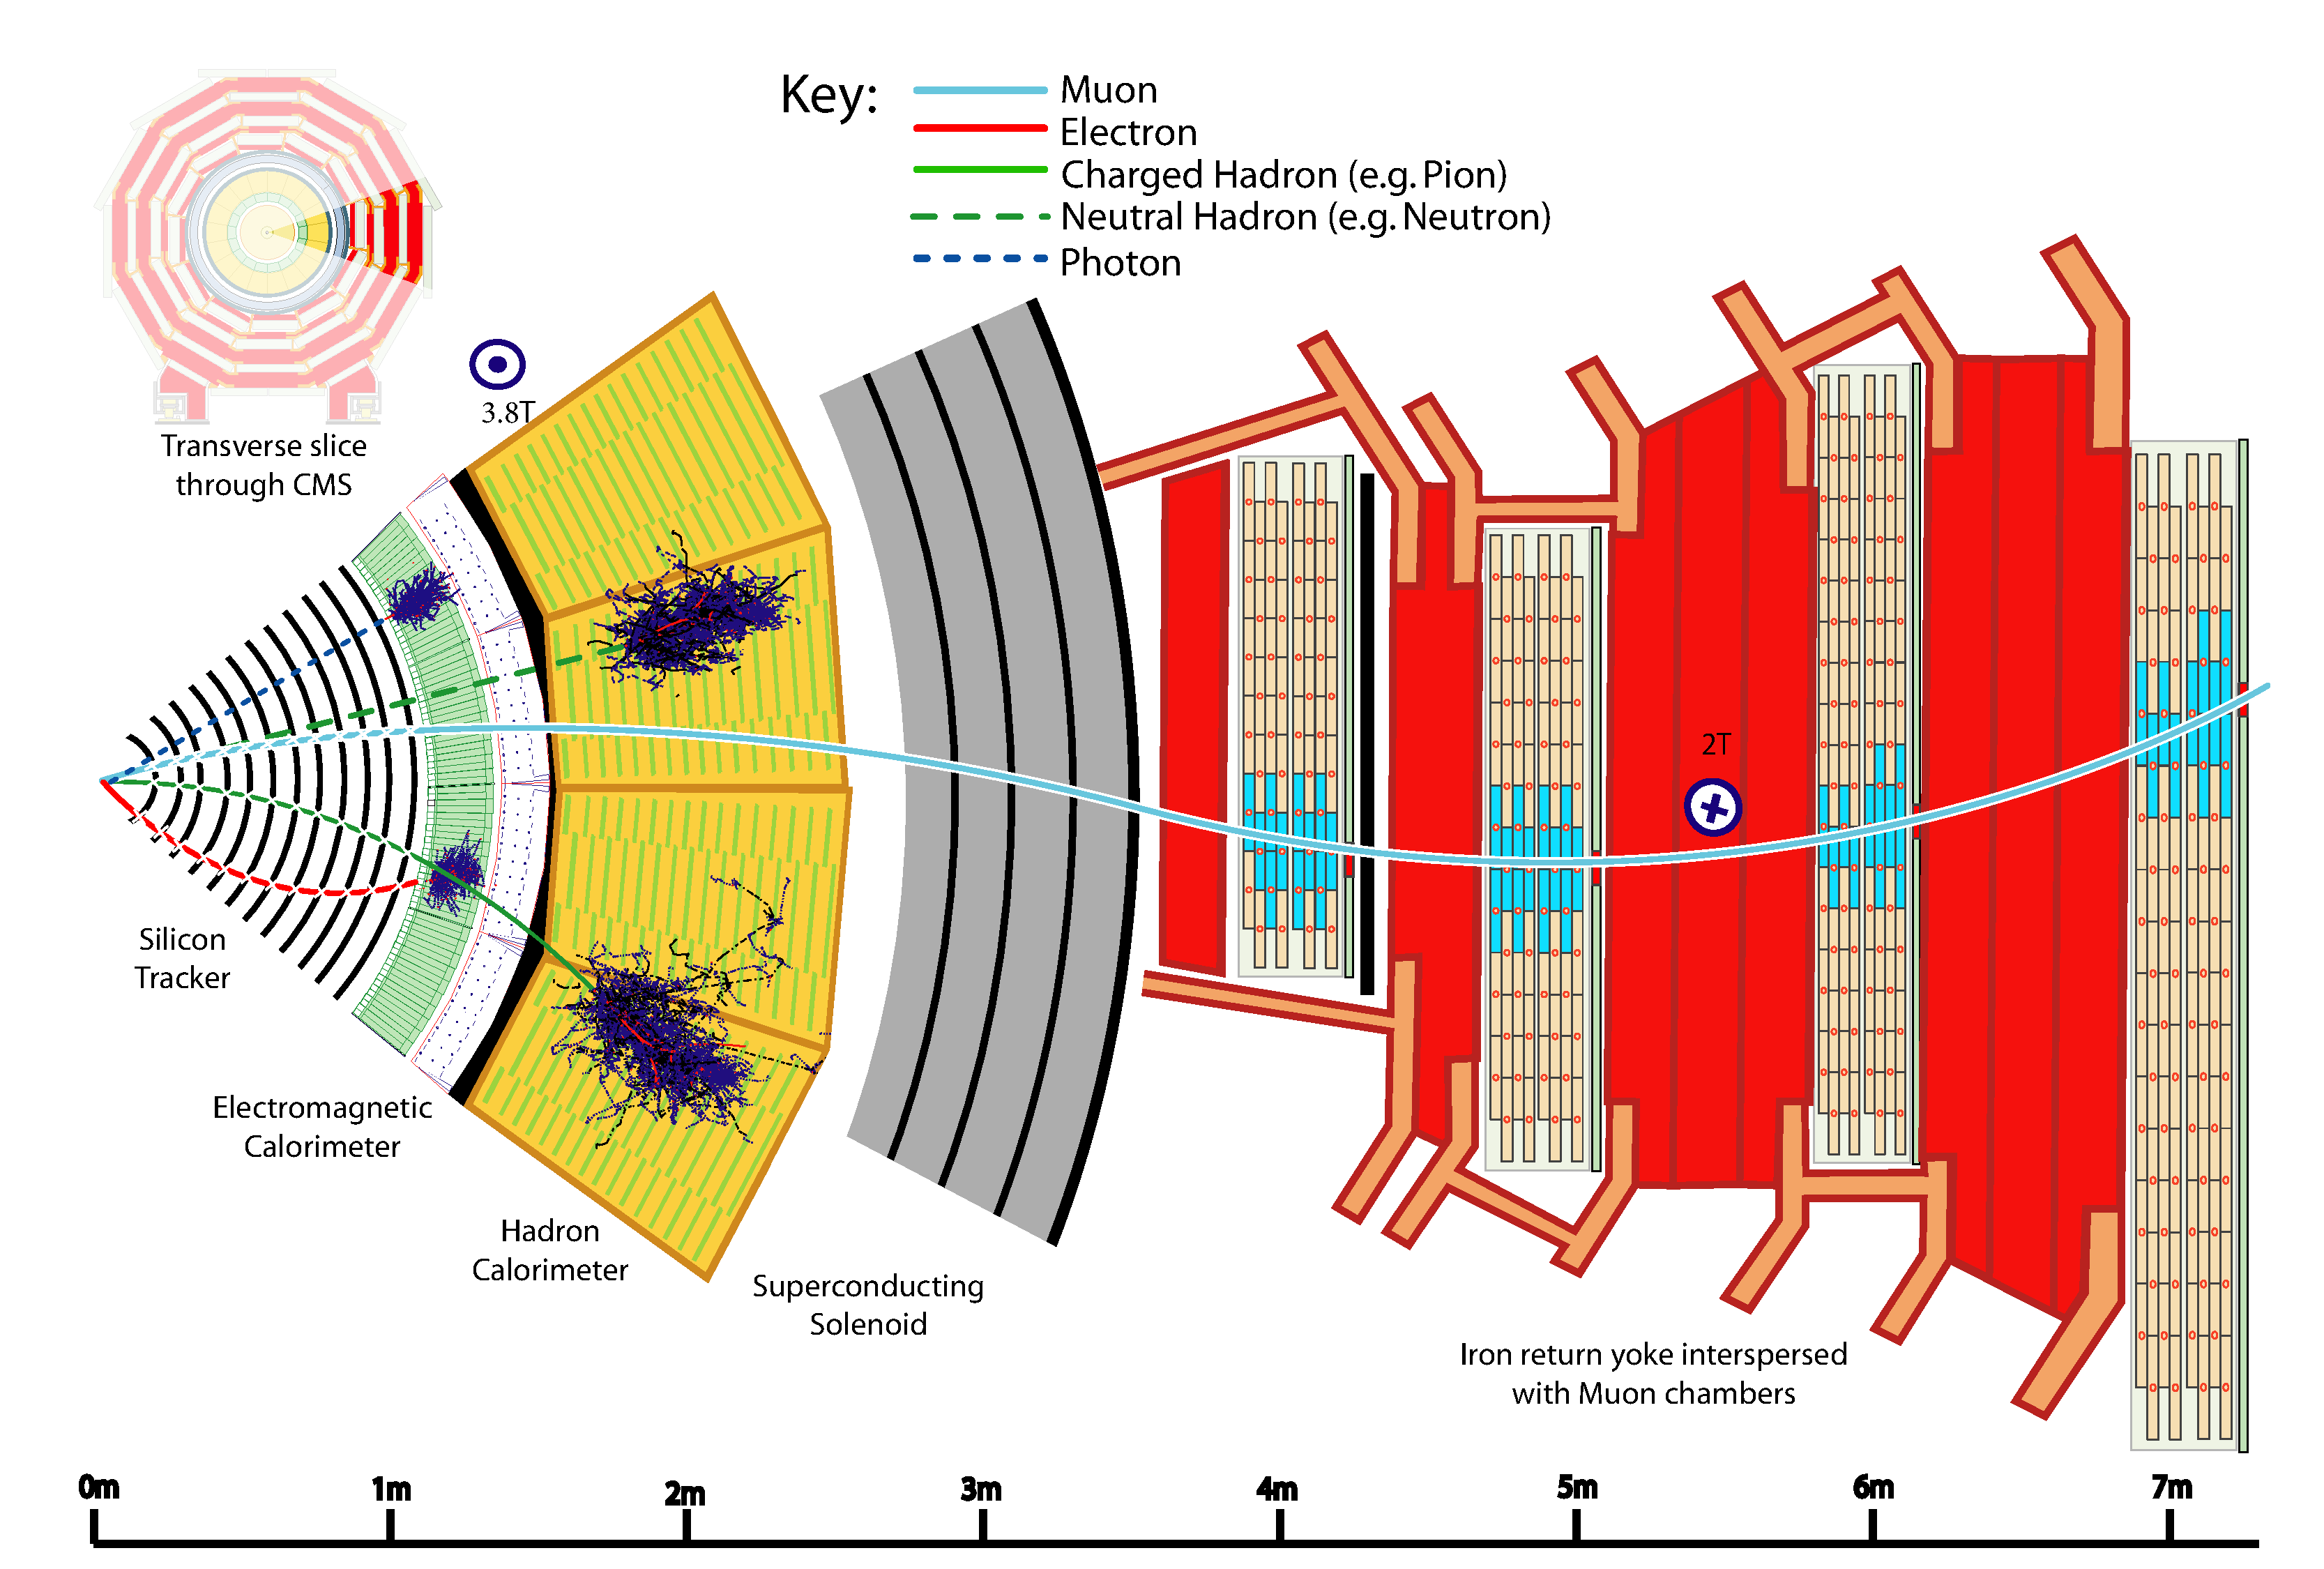
\includegraphics[width=\textwidth]{figures/particle_flow_detector.pdf}
    \caption[
        %Short caption for the list of figures
       Particle Flow in CMS.
    ]{
        % Full caption shown below the image
        Particle flow for some commonly observed particles in \CMS. The path of each particle and its detector response are shown diagrammatically here. By tying together information about each particle from the different subdetectors it travels through, an accurate calculation of its properties can be made.
    }
    % A label so you can \ref{fig:my_fig}. It is arbitrary; neither the 'fig:'
    % nor the fact that it has the same name as the pdf are required.
    \label{fig:particle_flow_cms}
\end{figure}

This analysis uses jets and muons to find candidate \WR events. Each of these requires several subsystems to be well-measured. For muons, the combination of hits in the tracker and the muon chambers is used to reconstruct the particle momentum. For jets, charged particles in the jets leave tracks, and all its components deposit energy in \ECAL and \HCAL. The combination of energies deposited in the two calorimeters are combined to estimate the jet energy.

With several proton-proton collisions occurring at the same moment, great care is taken to ensure that the components of jets all come from the same source. The tracker is used to identify which specific location each jet component comes from in the collision, called a vertex. The PuPPI algorithm is used to prune jets based on this. PuPPI is discussed further in section \ref{sec:jetreco}. Muons used in the analysis are also required to originate from the same vertex. 

\subsection{Tracker}

The tracker is at the center of \CMS and enables the reconstruction of charged particles passing through the detector from the collision point.  All particles travelling into \CMS with a \ensuremath{|\eta| < 2.5} from the interaction point pass through the tracker.  There are two main parts of the tracker: the strip tracker and the pixel detector, each made with silicon.  The strip tracker is used primarily for measuring momentum, and the pixel detector for position.
Silicon detectors operate by collecting ionized charge in material.  Each active layer in the detector gives an interaction location for the particle, which is related to the particle's momentum and charge. 

As the pixel tracker is closest to the beam line of all sub-detectors, just \ensuremath{\SI{4.4}{cm}} from the interaction point, it must also the highest position resolution.  Silicon was chosen to satisfy the stringent requirements of the detector. It has a very fast refresh time (faster than the time between interactions of \ensuremath{\SI{25}{ns}}), is radiation hard and pixels can be made small enough for the needed resolution.  

%The region closest to the interaction point is cylindrical and made up of several layers of pixel detectors, each \ensuremath{\SI{53}{cm}} long.  At higher \ensuremath{\eta} the orientation of the detector changes and is made up of several layers of discs.

%Each pixel in the tracker is just \ensuremath{100\times150 \mu m}.  Individual particle crossing positions are determined with weighted averages based on the amount of charge left in each pixel, which is also used for determining of the position beyond the pixel scale.  Charged particles bend in the magnetic field of \CMS angling their interaction with tracker, leading to more spread.

The strip tracker sits around and outside the pixel tracker.  The strip tracker allows for the determination of charged particles' momenta, by measuring their track curvature.  With the high magnetic field of \CMS and a longer distance from the interaction point, the measurement of momentum is improved over just the pixel detector. While a larger pixel detector could be built in the place of the strip tracker, this was not practical.  Each strip runs the length of a tracker module and is between 80 and 180 \ensuremath{\mu m} wide depending on its distance from the interaction. A cross-sectional view of the strip tracker can be seen in \ref{fig:tracker}.

\begin{figure}[!tp]
    \centering
    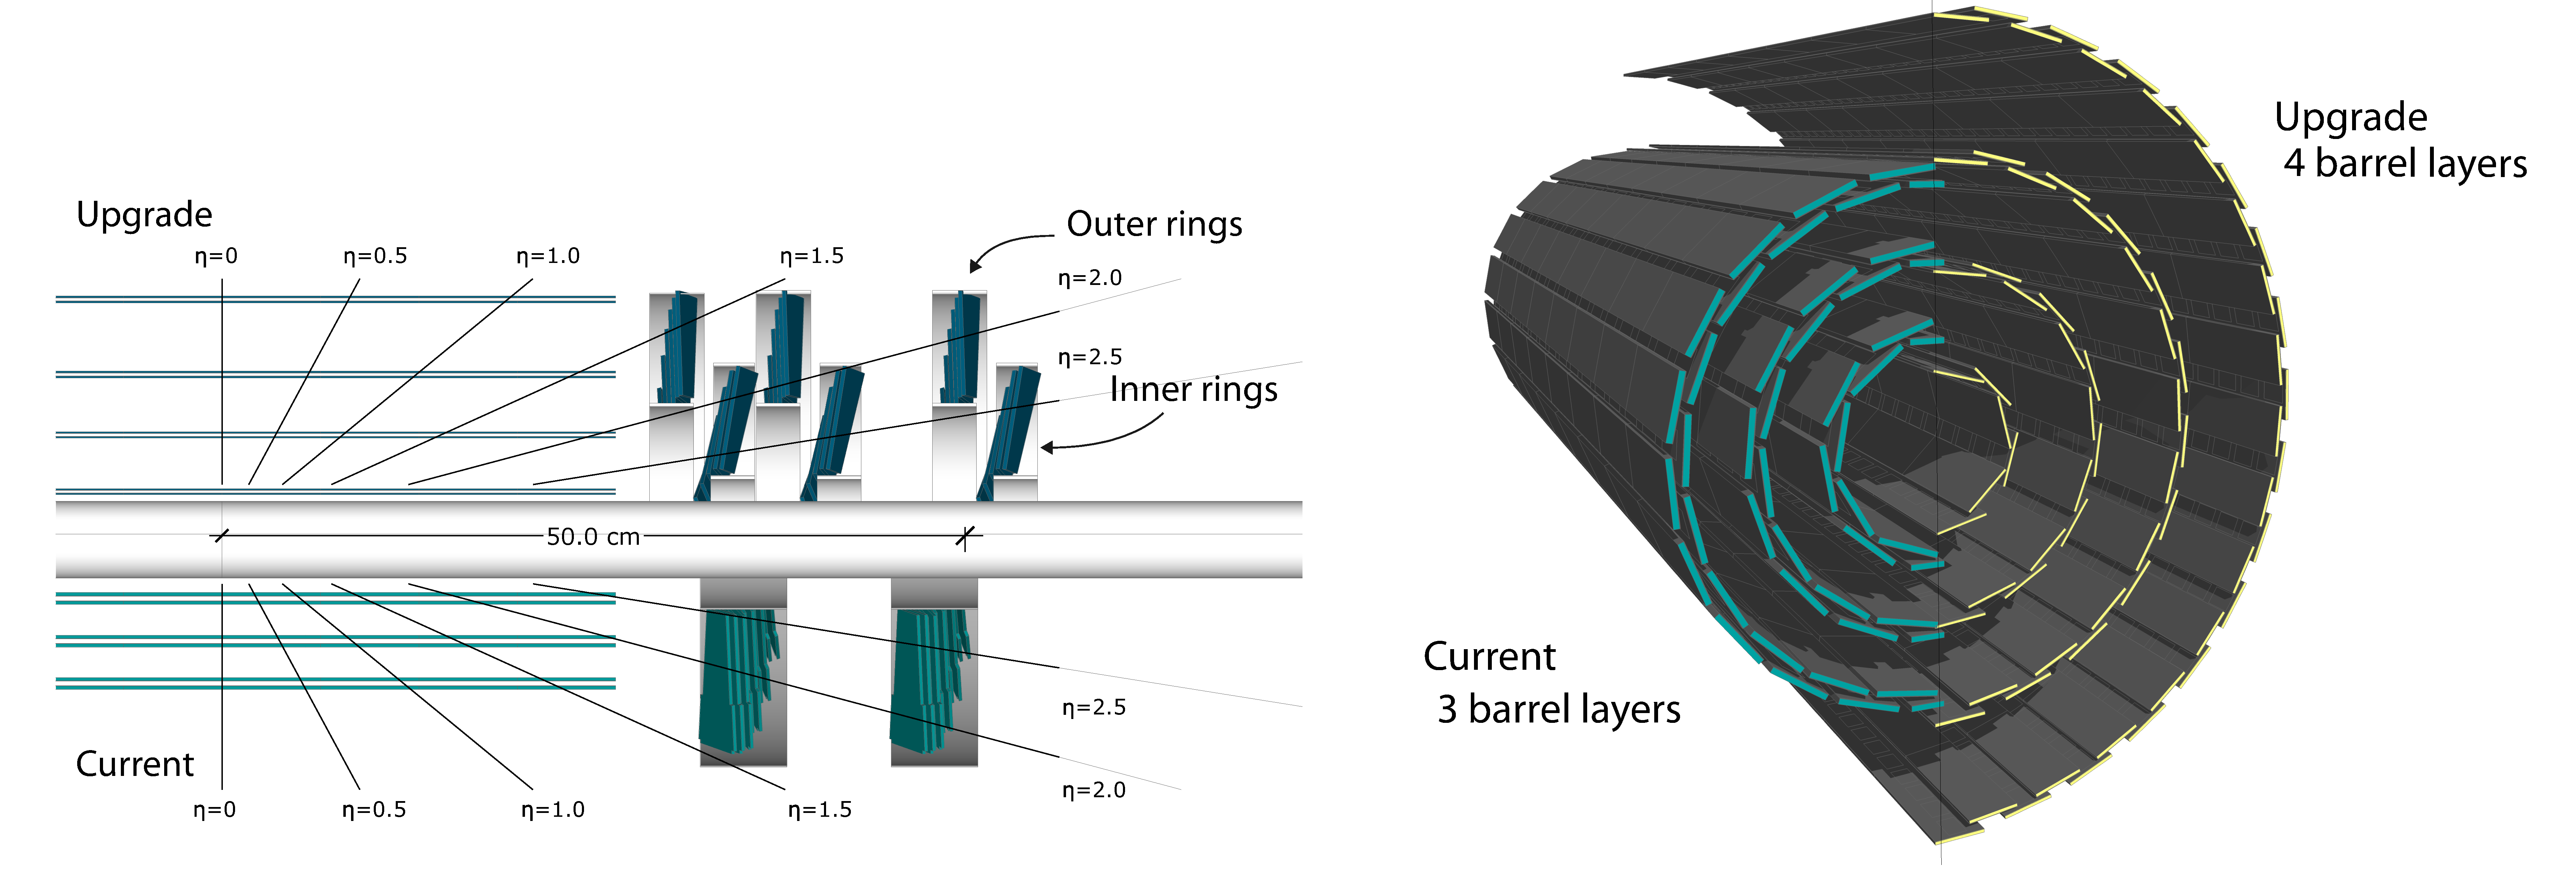
\includegraphics[width=\textwidth]{figures/tracker_layout_ng+og.pdf}
    \caption[
        %Short caption for the list of figures
       \CMS tracker diagram.
    ]{
        % Full caption shown below the image
        A cross-section of a part of the \CMS tracker is shown.
        On the left, a conceptual layout comparing the different layers and disks in the current and upgrade pixel detectors is shown. On the right, a transverse-oblique view comparing the pixel barrel layers in the two detectors can be seen.
        \cite{trackerPerf}
    }
    % A label so you can \ref{fig:my_fig}. It is arbitrary; neither the 'fig:'
    % nor the fact that it has the same name as the pdf are required.
    \label{fig:tracker}
\end{figure}

%One of the most significant challenges in using the tracker to its full potential is alignment. The position of the tracker components and the position of the tracker relative to the rest of \CMS must be known to better than the tracker's own resolution. This alignment calibration must be done completely in-situ and repeated at regular intervals. Cosmic-ray muons serve this purpose very well. Both with and without the magnetic field of \CMS turned on, the passage of these muons through the detector (and out the other side) allow for this alignment. Performance of the tracker is further understood using very well known standard model processes common in the proton-proton collisions at the \LHC. The \Ztomumu process is studied for this. The shape of the reconstructed mass of the \Z as a function of one of the muon's angle \ensuremath{\phi} reveals possible distortions in the tracker which can be corrected.

The precision of the tracker is ultimately key for identifying the primary interaction vertex in the event. This allows for the rejection of particles stemming from an uninteresting vertex (pileup). In the transverse plane its resolution is on the order of \ensuremath{\SI{100}{\mu m}} and longitudinally, \ensuremath{\SI{150}{\mu m}}. The resolution of a muon with \ensuremath{\SI{100}{\GeV}} of momentum is approximately \ensuremath{1\%} in the barrel region and \ensuremath{3-6\%} in the endcap region. For more information about the tracker see \cite{trackerPerf}.

\subsection{Electromagnetic Calorimeter}
WHY ECAL

The electromagnetic calorimeter (\ECAL) absorbs and measures the energy of charged particles passing through it. Electrons and photons are typically completely stopped in the \ECAL, while quark-matter particles will leave some energy and continue through to \HCAL. \ECAL is a total absorption calorimeter with an active material made out lead-tungstate crystals. Each crystal absorbs the energy of particles moving through by electromagnetic interactions, a fraction of the energy is then converted to scintillation light. The amount of light produced is then measured.

\begin{figure}[!tp]
    \centering
    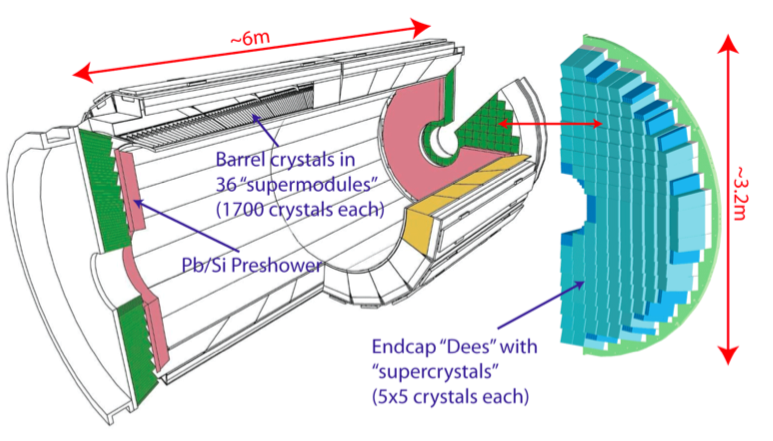
\includegraphics[width=\textwidth]{figures/ECAL_diag.png}
    \caption[
        %Short caption for the list of figures
       \CMS \ECAL diagram.
    ]{
        % Full caption shown below the image
        This cut-away of the \ECAL shows the barrel and endcap regions, as well as the pre-shower. Individual crystals and their alignment towards the nominal interaction point can be seen. \cite{ecalPerf}
    }
    % A label so you can \ref{fig:my_fig}. It is arbitrary; neither the 'fig:'
    % nor the fact that it has the same name as the pdf are required.
    \label{fig:ecal}
\end{figure}

\ECAL is divided into three sections covering all of \ensuremath{\phi} and out to an \ensuremath{\eta} of 3.0: The barrel (EB), end-cap (EE) and pre-shower sections (ES).  The barrel and end-cap have the same design, but with a different shape of the detector, though the crystals all still point near the interaction point at the center of \CMS. The \ECAL has a total of 61200 crystals in the barrel and 7324 crystals in the endcap. 
%As \ECAL is designed to surround the tracker, all of the power, readout, and cooling pipes for the tracker must pass through \ECAL somewhere. There is a gap between the barrel and endcap sections of \ECAL to allow for this. This gap is angled away from the interaction point to prevent particles travelling along it to be undetected.

Each crystal of lead-tungstate in \ECAL in the barrel region is \ensuremath{2.2\times \SI{2.2}{cm^2}} and \ensuremath{\SI{23}{cm}} long. In the endcap, they are slightly wider and shorter at \ensuremath{2.86\times \SI{2.86}{cm^2}} and \ensuremath{\SI{22}{cm}} long. These crystals are arranged in \fivebyfive groups arranged to be rectangular in \etaphi. The long axis of the crystals are misaligned by \ensuremath{\SI{5}{^\circ}} from the center of the detector. This reduces the chance that a particle travelling from the interaction point proceeds along the gap between crystals. 

%In additional to the crystals used in \ECAL, covering most of the endcap section is a part of the detector called the pre-shower. The pre-shower is a silicon detector which has much higher position resolution than the endcap section of \ECAL. The high spatial resolution was intended to improve the ability to determine the difference between single photons and boosted \pitogammagamma decays.

%condense the next two paragraphs??
\ECAL is the first usage of lead-tungstate, \leadtungstate, in a collider calorimeter. Lead-tungstate (as crystallized for \CMS) is clear, and its high density gives it a radiation length of just \ensuremath{X_0 = \SI{0.89}{cm}} and a Moliere radius of \ensuremath{\SI{2.2}{cm}}. Radiation lengths are a way of standardizing the amount of absorption that will occur in the detector. The Moliere radius is proportional to the volume over which the shower of energy spreads. The short radiation length of the crystal allows \ECAL to be smaller, and the small Moliere radius allows for higher spatial resolution in the detector.

The disadvantage of lead-tungstate is its low light yield with only \ensuremath{ ~\SI{30}{photons/\MeV}}. High-gain photo-sensors are used to amplify this signal.  The barrel region uses avalanche photo-diodes (APDs) and the endcaps use vacuum photo-triodes (VPTs).  Each has a high gain, while remaining relatively insensitive to the high magnetic field environment they operate in. Signals coming from each crystal are digitized and stored in electronics on the detector, and are only readout on request by the \CMS trigger system. This reduces the data rate for \ECAL, as sending all of the information for all crystals each collision was not be feasible in 2006, when the detector was constructed.
%%%
The best performance of \ECAL requires near-constant calibration. As with all detector components of \CMS, lead-tungstate is radiation resistant. However, the crystal structure is slowly damaged by radiation. Radiation creates imperfections in the crystal, reducing the light produced from an interaction. To maintain the highest possible precision, \ECAL is regularly recalibrated with a built-in laser system, which can operate during the abort-gap of the \LHC while collisions are underway.

\ECAL was first calibrated with dedicated beams and radioactive sources prior to being installed in \CMS.  With a known source, the whole detector was calibrated such that there is no asymmetry in the response based on \etaphi. The absolute calibration of the detector is also done with physics collisions in \CMS using the \Z boson. Its mass is very well understood from independent measurements and the signal is visible strongly over background.  The resolution is function of energy and is parameterized as:

\begin{equation}\label{eq:ecal}
    \frac{\sigma_{E}}{E}
    =   
    \frac{\SI{2.8}{\%}}{\sqrt{E/\left(\SI{1}{\GeV}\right)}}
    \oplus
    \frac{\SI{0.128}{\GeV}}{E}
    \oplus
    \SI{0.3}{\%}.
\end{equation}

More details on the performance of \ECAL can be found in \cite{ecalPerf}.

\subsection{Hadron Calorimeter}
\label{subsec:HCAL}
WHY HCAL

The hadron calorimeter (HCAL) sits outside the ECAL and samples the energy from hadrons produced in collisions.  The HCAL also stops most of the remaining particles, muons and neutrinos being the most common exception.

There are four sub detectors in HCAL: HCAL Barrel (HB), HCAL Endcap (HE), HCAL Forward (HF), HCAL Outer (HO).  These correspond to the barrel, endcap, forward and outer regions.  HB, HE and HO follow the same overall design.  Each is made out of layers of brass and plastic scintillator.  The brass is used to cause hadrons passing through to shower and it absorbs some of their energy. The energy of these showers is then measured in the subsequent plastic scintillator layer. Showers often pass through several HCAL layers before being totally absorbed.  The energy in each of these depths can then be summed for a total energy measurement, or compared to give more information on the shower evolution. A cross-section of HCAL with the regions HB, HE, and HO cover is shown in Fig.~\ref{fig:hcal}.

\begin{figure}[!tp]
    \centering
    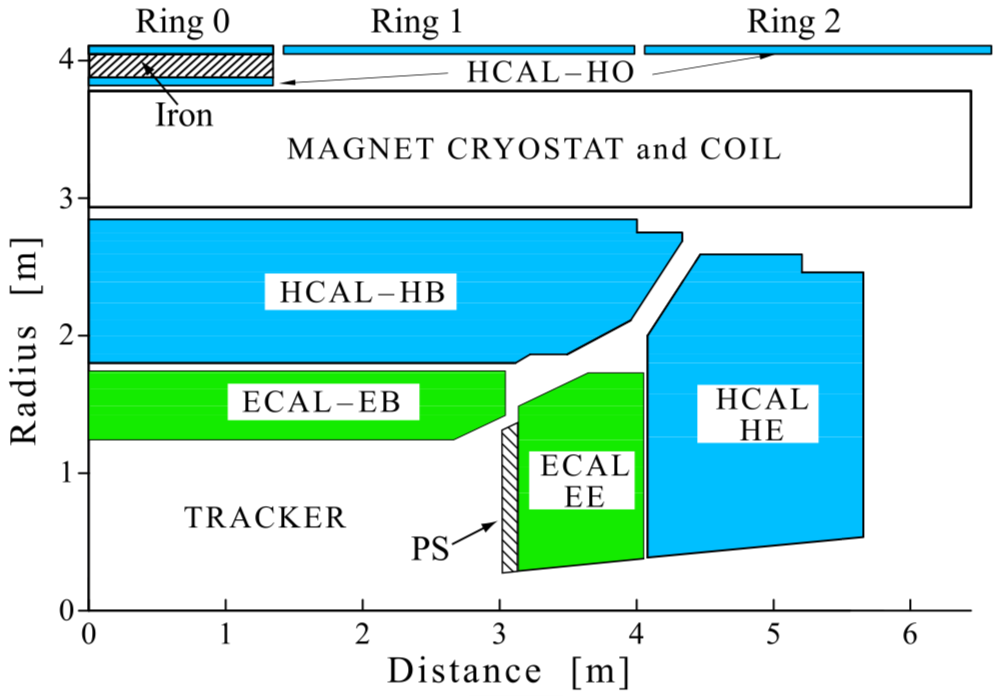
\includegraphics[width=\textwidth]{figures/HCAL.png}
    \caption[
        %Short caption for the list of figures
       \CMS \HCAL diagram.
    ]{
        % Full caption shown below the image
        This cut-away of the \HCAL shows the barrel and endcap regions, and it's arrangement with adjacent \CMS components.  The barrel and endcap regions are within the magnet. The gap between them allows for cabling to the inner detector. HF is not pictured as it sits separately in a higher \ensuremath{\eta}. \cite{HCALperf}
    }
    % A label so you can \ref{fig:my_fig}. It is arbitrary; neither the 'fig:'
    % nor the fact that it has the same name as the pdf are required.
    \label{fig:hcal}
\end{figure}

%The \CMS \HCAL, except HF, has 17 plastic scintillator layers each \ensuremath{\SI{3.7}{mm}} thick with the first and last layers thicker at \ensuremath{\SI{9}{mm}}.  In between each of the middle layers is brass absorber.  The outer layer being stainless steel.  The first layer is \ensuremath{\SI{61}{mm}} thick.  The eight layers after are thinner at \ensuremath{\SI{50.5}{mm}}.  The next six are slightly thicker at \ensuremath{\SI{56.5}{mm}}.  The last layer is the \ensuremath{\SI{75}{mm}}.  The initial layer's extra thickness helps catch showers which might begin in the gap between \ECAL and \HCAL, these would be impossible to reconstruct well.  The last layer is the thickest to attempt to stop any shower from continuing past \HCAL, though a few still will.  Outside of the \CMS magnet is another small layer, HO, meant to catch the most penetrating of showers.  Combining \ECAL and \HCAL, there are between 7 and 10 interaction lengths depending on the part of the detector.

HF is the most forward part of HCAL and the most forward detector used in event reconstruction.  It covers the \ensuremath{|\eta|} of up to 5.0.  As a result of the significantly higher particle flux in the forward regions, HF has a special, exceptionally radiation hard design. The bulk of HF is comprised of steel, with quartz fibers running horizontally through it. These quartz fibers measure the energy of particles passing through them by the direct Cerenkov radiation produced in them. Each channel in HF comprises two bundles of such fibers, one short and one long. The long fibers run the length of HF, whereas the short fibers end farther from the inward side. The difference between the energy deposited in the fibers can be used to determine how deeply the transiting particle showered, which is related to whether the particle is a photon or lepton as opposed to a hadron, which will shower deeper into the detector.

\HCAL has been specifically designed to measure the energy of hadrons.  Hadrons detected by \HCAL are generally pions, which are light quark anti-quark pairs.  Neutral pions decay quickly and to leptons, which is well absorbed in \ECAL.  Charged pions, however, decay more slowly, via the weak-force. These, as well as neutrons and protons, pass through \ECAL.  Any electrically charged hadron will interact with the tracker and \ECAL, leaving only some energy, as they are much heavier than electrons, with the same magnitude of charge. Hadrons will, however, interact via the strong force with nuclei in the detector. This happens in \ECAL as well as \HCAL. Each interaction can create more hadrons with energy sufficient to continue travelling through the detector. The energy of a hadron initially interacting with the detector is then distributed throughout \ECAL and \HCAL and requires a more careful reconstruction.

The specific ratio of neutral and charged pions involved in a shower is inherently random.  Each shower will contain different amounts.  Since each shower is started by only tens of hadrons, these fluctuations can be significant.  The calorimeters do not have the same response to the electromagnetic interactions from neutral pion decays and the nuclear interactions of charged pions.  This results in a degraded resolution of \HCAL from what might be theoretically expected.  The behavior of the detector response with respect to different hadrons, and the distributions of them in a shower have to be understood to make accurate measurements.

Signal amplification from the plastic scintillators was originally done with hybrid photo-diodes.  These are in the process of being replaced, however, with silicon photo-multipliers (SiPMs).  SiPMs offer improved resolution improving detector performance despite radiation degradation of the scintillator.  The forward part of \HCAL, HF, is much more removed from the magnetic field environment and continues to use photo-multiplier tubes.

Before installation, parts of \HCAL was fully assembled along with \ECAL and tested with pure electron and pion beams.  These tightly controlled beams allowed for the \ensuremath{\pi / e} correction to be derived and the detector response calibration.  As with all sections of \CMS, radiation damage is problematic and requires continual study.  \HCAL does not require the same level of calibration as \ECAL, but still uses a laser system, operating within and outside of physics data taking to monitor detector performance.  The original resolution of \CMS \ECAL and \HCAL combined for hadronic particles is:

\begin{equation}\label{eq:hcal}
    \frac{\sigma_{E}}{E}
    =   
    \frac{\SI{84.7}{\%}}{\sqrt{E/\left(\SI{1}{\GeV}\right)}}
    \oplus
    \SI{7.4}{\%}.
\end{equation}

As can be seen in equation \ref{eq:hcal}, hadronic particle energy reconstruction does not have near the resolution as electrons and photons. 

\subsection{Muon Chambers}
WHY MUONS

The muon chambers detect muons passing through and out of the detector. The muon detectors, in conjunction with the tracker, allow for the momentum of the muons to be measured very accurately. As the radius of curvature of muon tracks is proportional to their momentum, with sufficiently low momentum muons (generally \ensuremath{p_T < \SI{200}{\GeV}}) the tracker is sufficient for determining the momentum.  However, the straighter tracks of higher momentum muons benefit greatly from the additional information from the muon system. Sitting outside the \CMS magnet, all particles, other than neutrinos, are absorbed prior to reaching the muon detectors.  By connecting tracks with the muon detectors, muon identification can be performed in a straightforward manner.

The muon chambers are further from the interaction point than any other endcap or barrel detector.  They cover an area of roughly \ensuremath{\SI{25,000}{m^2}}.  Depending on the specific region of the detector, one of three technologies is chosen.  In the barrel section, the detectors are drift tubes (DT) and resistive plate chambers (RPC).  The RPC is used additionally in the endcap along with cathode strip chambers (CSC).  CSCs continue to highest rapidity region of the muon detector.  A diagram of the layout of the muon chambers is shown in Fig.~\ref{fig:muonchambers}.

\begin{figure}[!tp]
    \centering
    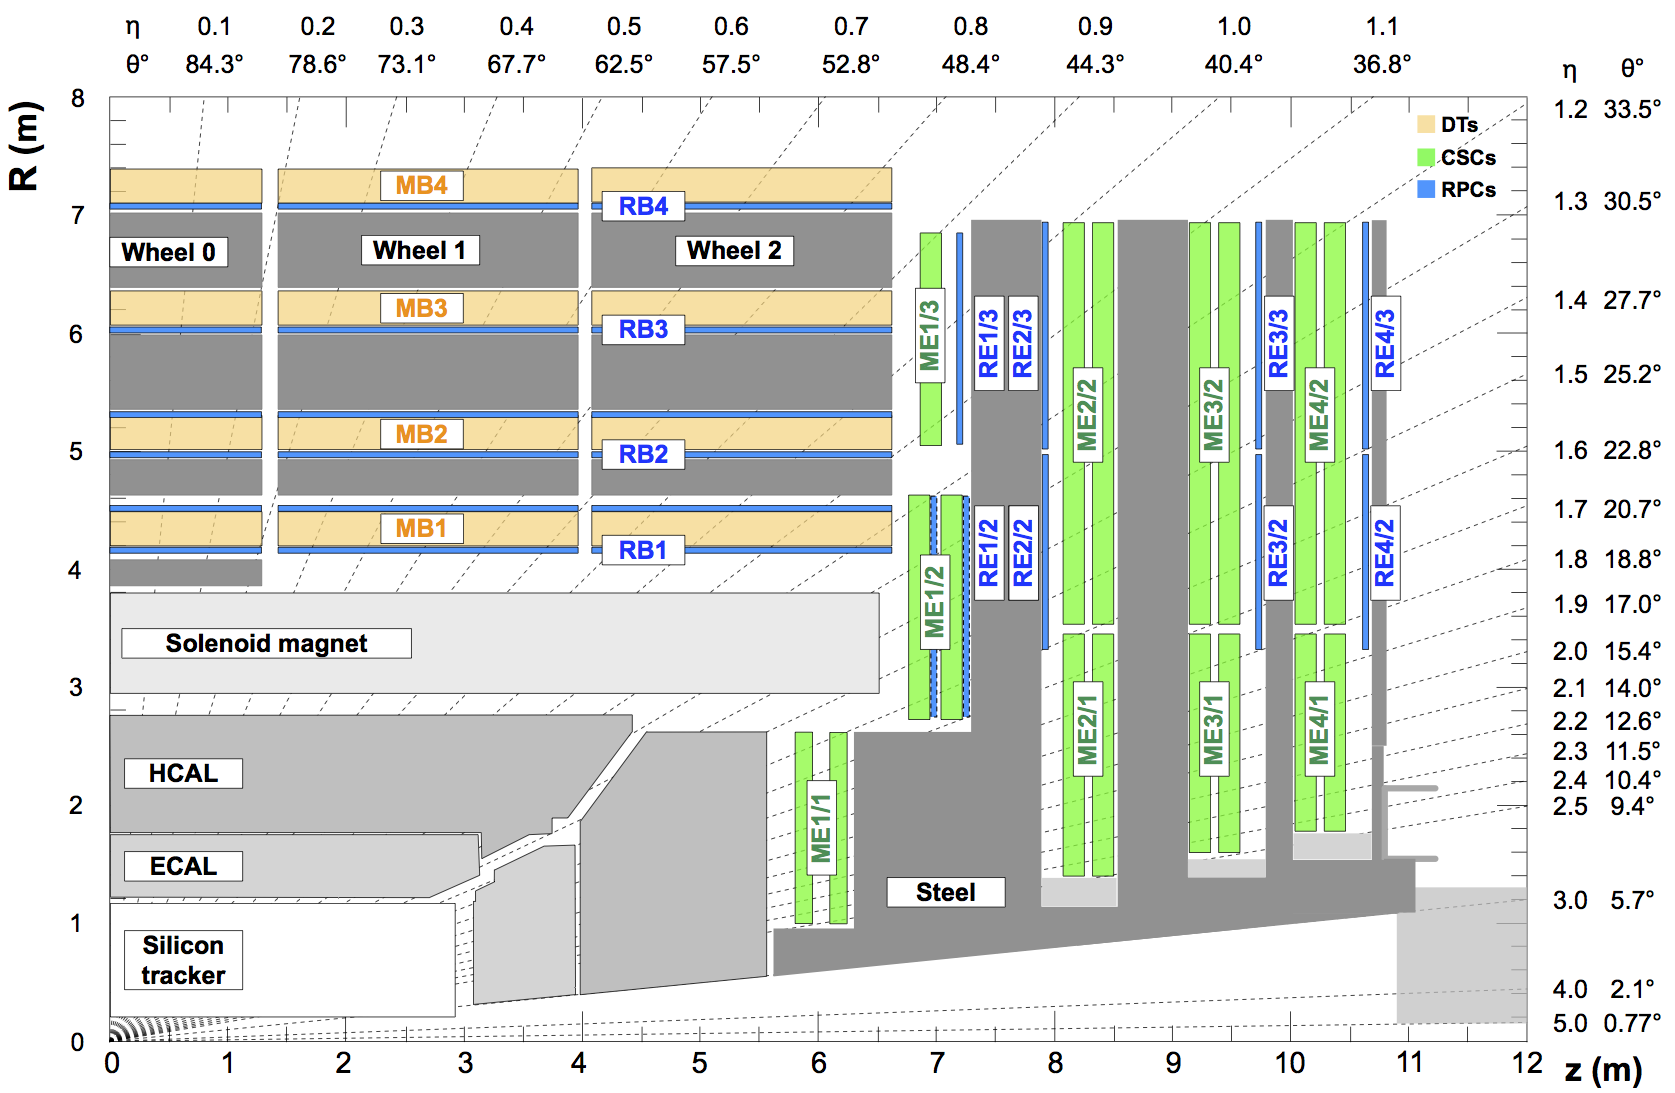
\includegraphics[width=\textwidth]{figures/muonSystem.png}
    \caption[
        %Short caption for the list of figures
       \CMS muon chambers diagram.
    ]{
        % Full caption shown below the image
        This cut-away of the muon system shows the barrel and endcap regions, and its arrangement with adjacent \CMS components.\cite{muonDPG13TeV}
    }
    % A label so you can \ref{fig:my_fig}. It is arbitrary; neither the 'fig:'
    % nor the fact that it has the same name as the pdf are required.
    \label{fig:muonchambers}
\end{figure}

DTs are a type of gas ionization detector.  Muons passing through gas ionize molecules, these ions are collected by an anode wire running down the center of the tube, the body of which functions as a cathode.  The timing and shape of the current in anode as it collects charge allows for a determination of the position of the muon as it passed through.  The barrel part of the muon system contains for layers of DTs.  These layers are separated by the iron return yoke of the magnet and each contains either 12 or 18 layers.  The alignment of the tubes in the first of the three sets is such that position in the \rphiplane and along the \ensuremath{z} direction can be measured.  The outer layer just measures in the \rphiplane.

In each of the four layers of DTs, RPCs are installed for improved performance.  RPCs have worse position resolution that DTs, but a faster response time, as the ionized particles drift a smaller distance.  RPCs contain two parallel plates of resistive material.  A high-voltage is setup across the plates and gas fills the gap.  Muons passing through this gap create ionizing particles.  The electrons from this ionization drift to the strips of anodes in each RPCs.  As the muons travel from the interaction point at roughly one foot per nanosecond, they may not exit the detector before the next interaction has begun.  The timing of the muon interactions as it passes through must be known precisely.  The response time of the RPCs is ~\ensuremath{\SI{1}{ns}}, much smaller than the time between a bunch-crossing.

In the endcap region, the magnetic field can be higher strength, and have a more complicated shape as the field lines connect through the solenoid. This, along with the higher particle flux in this region, creates challenges necessitating another design for muon measurement. CSCs are used instead of DTs. CSCs are a relatively flat gas chamber with anode and cathode wires running orthogonal and on opposite faces. The signal time at the anode is relatively prompt and can be used for the \CMS trigger system. The charge on the cathode stripes gives a more precise particle position, but is too slow for triggering. RPCs are also in the endcap for further performance. The endcaps have three layers of CSCs and RPCs with iron return yoke in between. Each CSC layer has six slices, giving excellent muon position and direction measurements.  Beyond \ensuremath{|\eta| > 1.6} the endcap only has CSCs. A complete discussion of the muon detector system performance can be found here \cite{muonDPG13TeV}.

\subsection{The Magnet}
The central solenoid magnet of \CMS is a critical component of the detector. It produces a magnetic field of \ensuremath{\SI{3.8}{T}} throughout the barrel regions of the tracker, ECAL, and HCAL, with an internal diameter of roughly \ensuremath{\SI{7}{m}}. Any larger, and the magnet could not be delivered to the \CMS site upon assembly. It also produces a \ensuremath{\SI{2}{T}} field within the iron return yoke surrounding and supporting the muon chambers. The superconducting material is niobium-titanium, embedded in aluminum, with \ensuremath{\SI{18000}{A}} of current running through it. This results in a stored energy of approximately \ensuremath{\SI{2.66}{GJ}}. The magnetic field exerts a force on charged particles according to their momentum perpendicular the magnetic field, which bends their paths. This allows for particle charge to be distinguished, as well as momentum measurement based on the radius of the track.  Once constructed, the cosmic ray measurements with the muon system allowed for precision understanding of the magnetic field throughout the detector.  \cite{magnet}.

\subsection{The Trigger}

The \LHC delivers collisions at \ensuremath{\SI{40}{MHz}}. Only 1 in 400,000 can be written to disk. The complicated task of deciding whether an event is worth keeping is given to the trigger system. The \CMS trigger system is comprised of two layers: a hardware level trigger designed to handle the full \ensuremath{\SI{40}{MHz}} of events and filter it down to \ensuremath{\SI{100}{kHz}} called the level one (L1) trigger, and the high level trigger (HLT) which is operated by a computer farm which further reduces the rate to \ensuremath{\SI{100}{Hz}}.

The L1 trigger is designed to be able to make trigger decisions very quickly, as the new events continue to come in, and to have as little latency as possible, as the more latency, the more information must be cached in the hardware prior to readout.  As a result of these constraints, the L1 trigger can only perform simple and regional calculations to determine an event's characteristics.  The \ECAL and \HCAL calculate basic information about the detector signals and give this information to the global trigger (GT).  At the same time, the muon sub-systems calculate trigger information to pass to the GT as well. With this combined information events are saved based on the total information available.  From here, a signal, level one accept (L1A), is sent to all the relevant detector hardware. The total event information, stored in a hardware pipeline, including the tracker systems, is sent to the HLT for further decisions. This happens on the order of microseconds.

The HLT software is run by roughly 10,000 CPU cores.  Each event, which is several megabytes, with its full information available to the HLT, must be understood to winnow and keep just 1 in 1000.  To do this, simple trigger paths, which are categories an event may fall into which would make it worth keeping, are calculated first.  After simpler paths are exhausted, more complicated calculations have time to be made.  Once an event passes an HLT trigger path it is immediately saved and the next can be analyzed.  The software running on the HLT computers is the same as that used by the final reconstruction software.  This allows full access to any algorithms used in the software.

The trigger system at \CMS is able to be reconfigured easily, and is continually studied and improved to maximize its efficiency in selecting worthwhile events, and to prevent unintentional biasing of the saved data.
With the total delivered luminosity of \GLNTOTALII , \CMS has saved petabytes of collision data from the second run.

\section{The HCAL Phase I Upgrade}
\subsection{Overview}
The Hadronic Calorimeter for \CMS as discussed in section \ref{subsec:HCAL}, is critical in the measurement of hadronic activity in the detector and electron and photon identification. As the detector has aged, primarily from radiation during beam collisions, the performance of the plastic scintillator has decreased. In addition, the original \HCAL design had limited bandwidth with the result of this being the energies recorded in several layers of plastic scintillator being summed to make depths.  With more bandwidth, more layers can be recorded individually. Upgrading the light gathering sensitivity of the detector, as well as increasing the bandwidth of information moving off detector, gives \HCAL the ability to increase its performance to low-energy events even with the lower light yields of the damaged scintillator.  The detector also has more depth information, by summing layers of plastic scintillator into more regions. With additional depth information, each layer of \HCAL can be individually calibrated. This improves performance especially as parts of the detector closer to collisions are radiation damaged more quickly. The number of depths in \HCAL before and after the phase I upgrade is shown in Fig.~\ref{fig:HCALdepthsRunI} and \ref{fig:HCALdepthsPhaseI} respectively.

\begin{figure}[!tp]
    \centering
    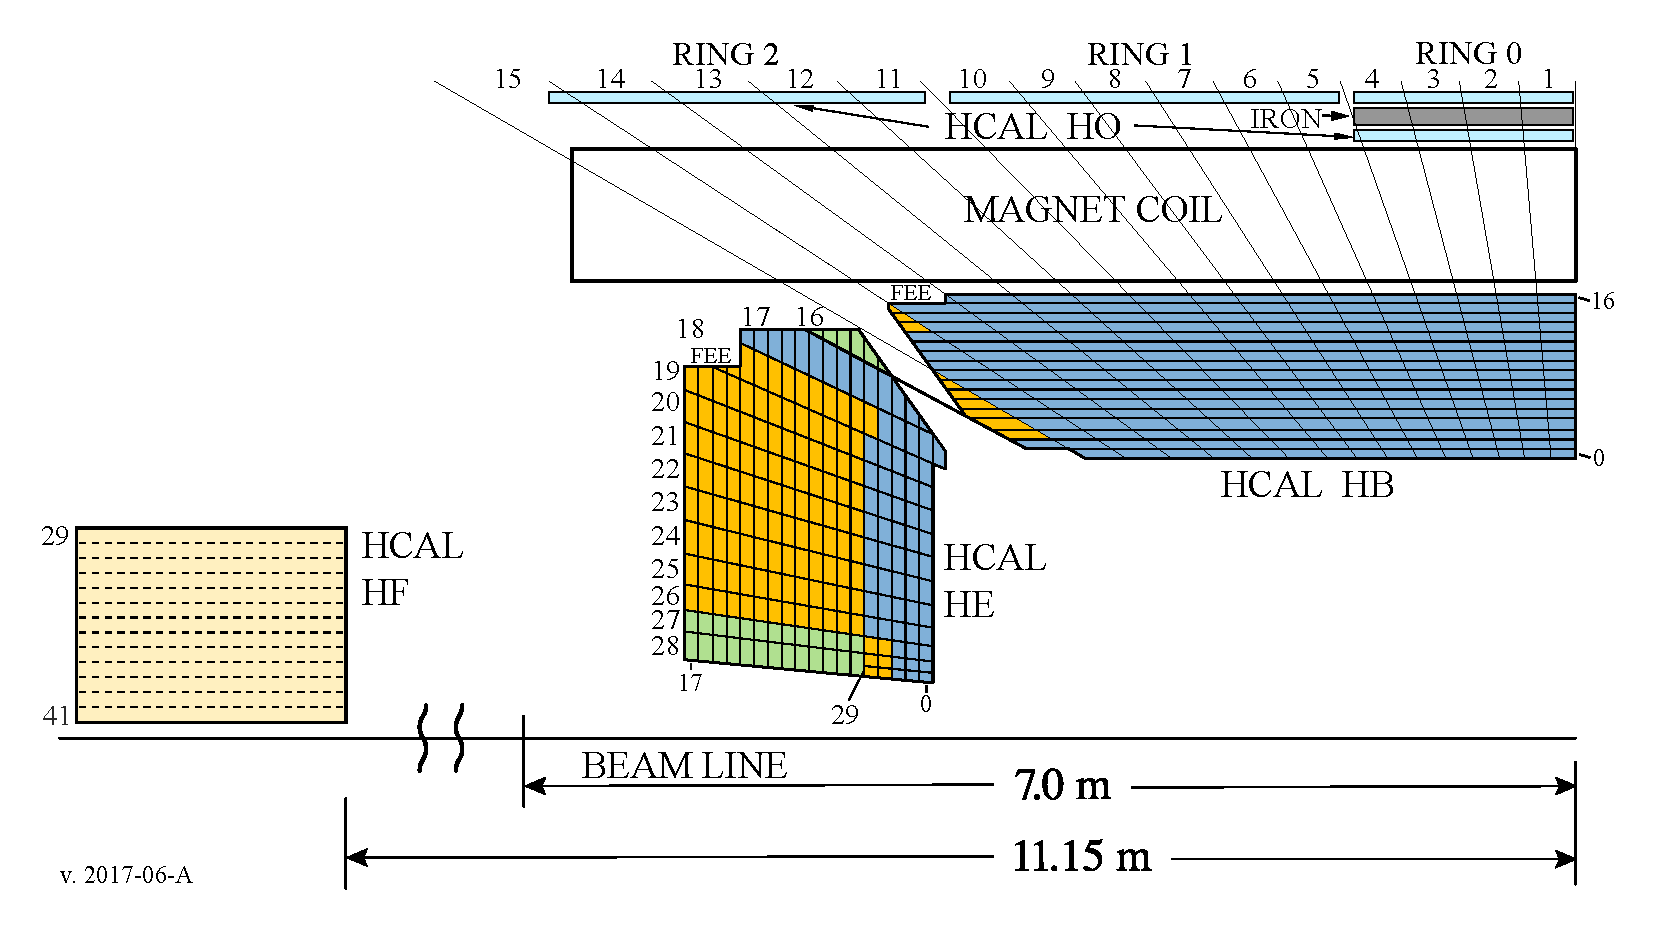
\includegraphics[width=\textwidth]{figures/HCAL-Depth-Segmentation-Legacy-View-HBHEHFHO-v201706A.pdf}
    \caption[
        %Short caption for the list of figures
       \HCAL legacy depth segmentation.
    ]{
        % Full caption shown below the image
        The Run I depth segmentation used by \HCAL.  It can be seen that the majority of \HCAL is summed into one or two depths.
    }
    % A label so you can \ref{fig:my_fig}. It is arbitrary; neither the 'fig:'
    % nor the fact that it has the same name as the pdf are required.
    \label{fig:HCALdepthsRunI}
\end{figure}

\begin{figure}[!tp]
    \centering
    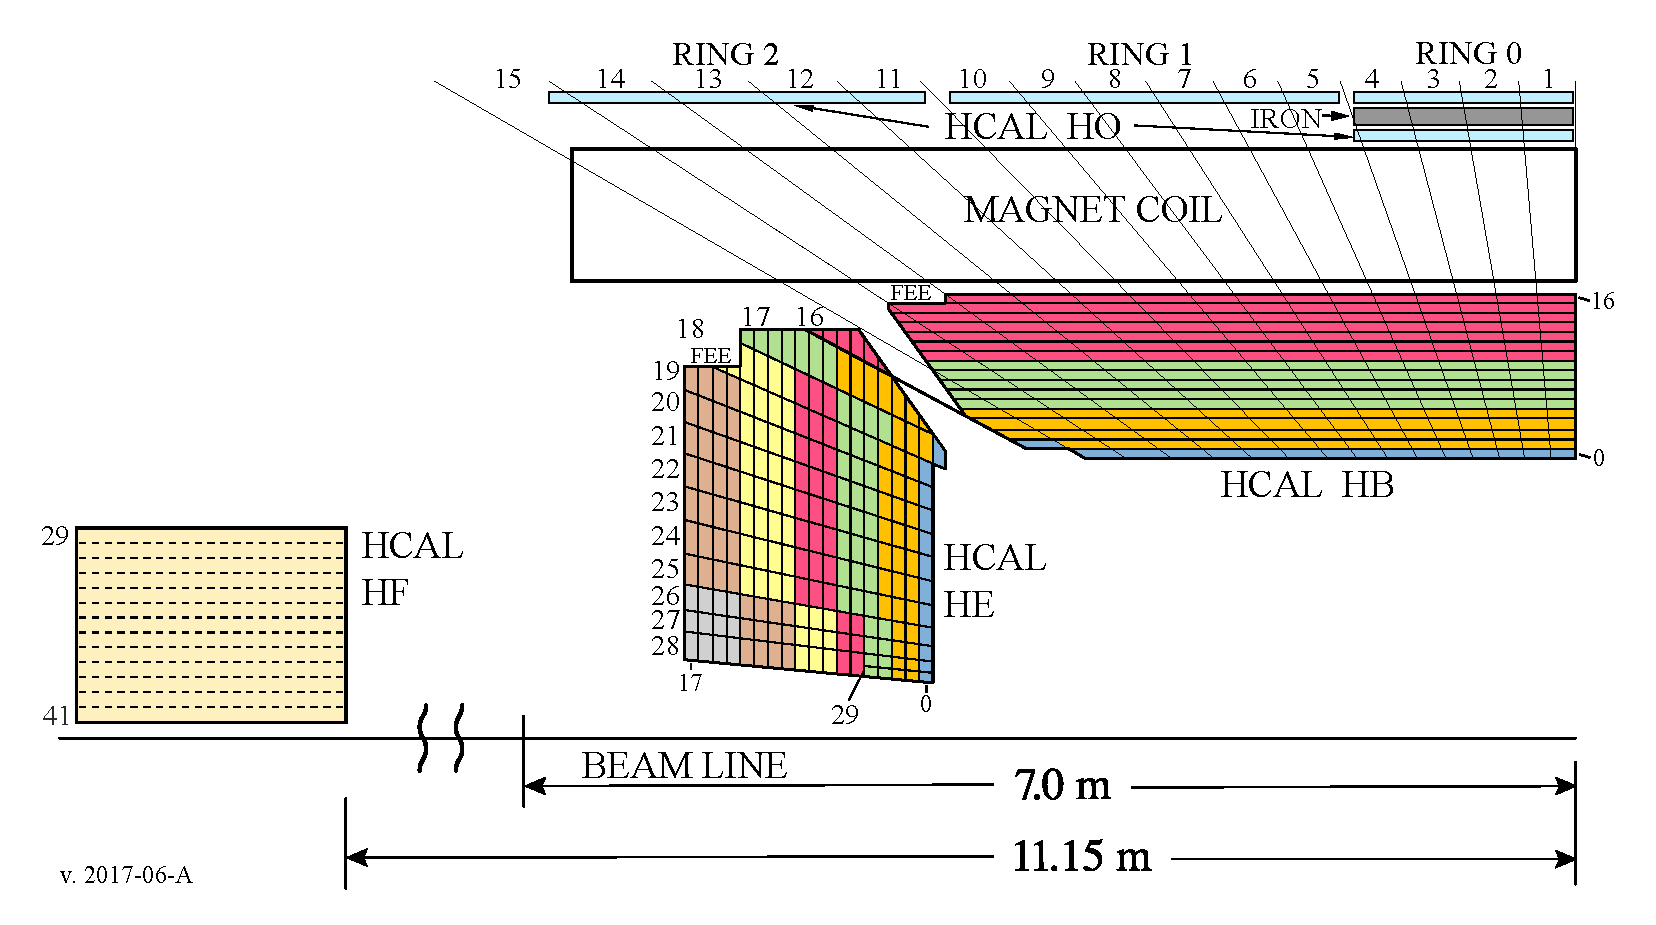
\includegraphics[width=\textwidth]{figures/HCAL-Depth-Segmentation-Phase1-HBHE-View-HBHEHFHO-v201706A.pdf}
    \caption[
        %Short caption for the list of figures
       \HCAL phase I upgrade depth segmentation.
    ]{
        % Full caption shown below the image
       The complete phase I upgrade \HCAL detector depth segmentation.  Several more depths are available throughout \HCAL. 
    }
    % A label so you can \ref{fig:my_fig}. It is arbitrary; neither the 'fig:'
    % nor the fact that it has the same name as the pdf are required.
    \label{fig:HCALdepthsPhaseI}
\end{figure}

\subsection{Front-End Control}
With the upgrade of the \HCAL detector readout capabilities came a desire to redesign the on-detector electronics control system.  We'll give an overview of the hardware involved in the front-end control system, and then discuss the software elements involved in each piece. The goal of the new system was to manage the large amount information needed to monitor and conFig.~the detector hardware in a robust way.  Here the author will make a brief detour to discuss these changes and one issue, important to the analysis, which occurred as a result.
\subsubsection{Hardware Layout}
A natural way to organize the hardware involved in the \HCAL front-end control system is to distinguish between components on the detector, and components off the detector.  \CMS has two caverns, called the service cavern (USC) and the experimental cavern (UXC).  The service cavern is protected from the radiation and magnetic field environment of \CMS and contains the majority of the controlling hardware, from PCs in racks to power-supplies and custom detector readout electronics.  UXC is almost entirely filled with the actual \CMS detector and includes some cooling and power supplies as well as any electronics required to amplify and digitize any detector signals.  By necessity, these electronics are specially selected for each region of the detector to fit the constraints of not just enduring the high magnetic field and ionizing radiation, but also a compact size and reasonable power consumption.

In the front-end, the \HCAL electronics are divided into readout boxes (RBXs). Each RBX contains the electronics necessary to digitally process the signals from scintillator. In parts of \HCAL with SiPMs, these are also contained in the RBX. For HF, the RBXs are located in racks adjacent the detector, and process signals from the PMTs. For the \HCAL phase I upgrade, each RBX contains an next-generation Clock and Control Module (ngCCM).  The ngCCM receives and sends all fast and slow control through each RBX over a backplane.  The ngCCM communicates with the USC side electronics through the next-generation Front-End Control Card (ngFEC).  Each RBX contains several charge integration and digitization chips (QIEs) as well as a calibration unit (CU). Each ngFEC sits in a uTCA crate in USC.  From here, it receives fast control messages from the trigger and clock distribution system (TCDS) and communicates with the ngCCM server, which will be discussed in \ref{sec:HCALphaseI_control} via IPbus.  Data from the front-end is sent to back-end crates to FPGA based models called uHTRs. A diagram for the next-generation front-end system is shown in Fig.~\ref{fig:HCALngFElayout}.
\begin{figure}[!tp]
    \centering
    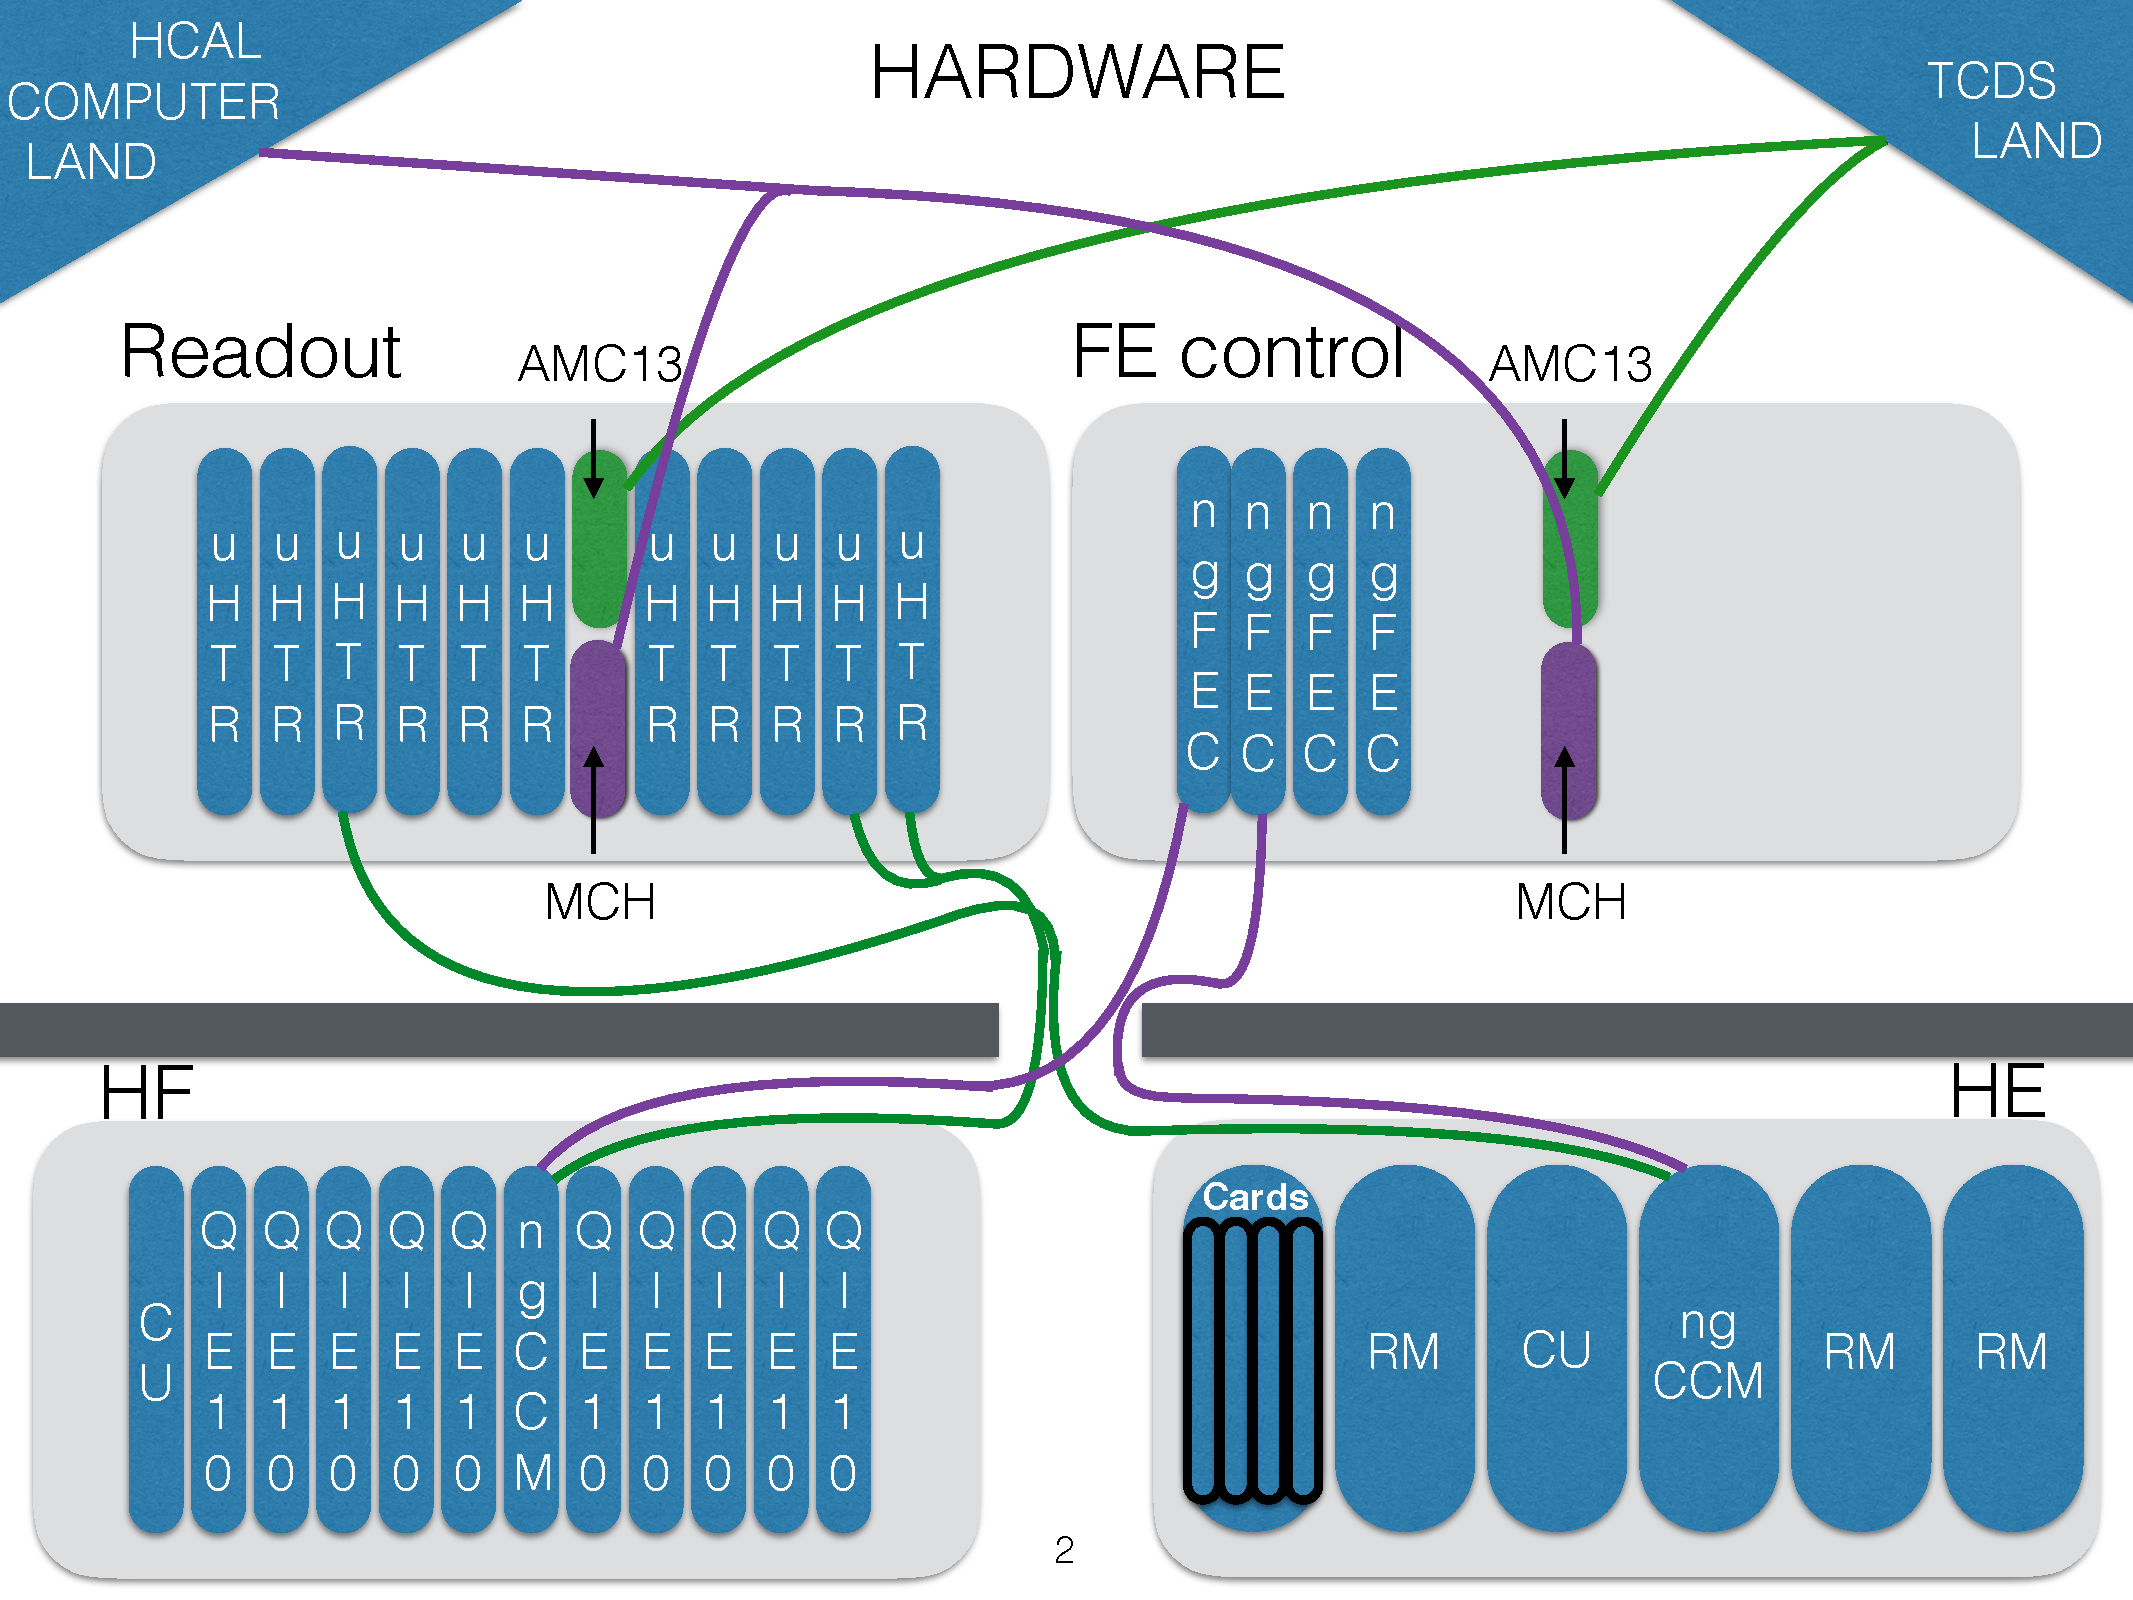
\includegraphics[width=\textwidth]{figures/HCALngFElayout.pdf}
    \caption[
        %Short caption for the list of figures
       \HCAL Phase I Upgrade Control and Readout Layout.
    ]{
        % Full caption shown below the image
        In the upper part of the diagram, the \HCAL and computer system and TCDS are shown.  These connect with back-end readout crates, containing uHTRs, and frontend control crates containing ngFECs.  These crates sit in USC.  The AMC13 and MCH are one to a crate and handle communication with various components over the crate backplane. From USC to UXC fiber optic cables for fast and slow control and detector readout sit.  In the front-end, there are different RBXs layouts for the different \HCAL subdetectors.  The QIEs, and there bundling in RMs in HE are shown, along with the CU and ngCCM.
    }
    % A label so you can \ref{fig:my_fig}. It is arbitrary; neither the 'fig:'
    % nor the fact that it has the same name as the pdf are required.
    \label{fig:HCALngFElayout}
\end{figure}
\subsubsection{Software Control}
\label{sec:HCALphaseI_control}
The software control system is designed around a single application forming the hardware to software interface.  This is called the \texttt{ngCCM server}. Other specific applications interface with the server, and reside in the \HCAL application framework for handling specific tasks.
The \texttt{ngCCM server} communicates with each ngFEC over IPbus.  Its communications are either directly with the ngFEC, or are forwarded to an ngCCM over one of the two I2C links.  The server has three client interfaces. The first is over websockets which sends and receives text strings in communication with the server, this link allows communication with \HCAL online software applications, and it is extensively used by an application called \texttt{ngRBXmanager}.  The second client interface is used by the detector control and safety (DCS) system.  DCS is responsible for managing power, cooling, and any other physical needs, as well as monitoring for any hazards.  The third client interface is a command line interface program which is primarily used by hardware and software experts.  A control scheme showing the various applications can be seen in Fig.~\ref{fig:ngFESW}.

The \HCAL online software applications communicate with three primary purposes.  \texttt{ngRBXmanager} is responsible for taking \HCAL configuration files and generating \texttt{ngCCM server} websocket client commands. These are sent when the detector is configured for data taking. The \texttt{ngRBXmanager} also ensures that the \texttt{ngCCM server} is properly working and its configuration of the detector was successful. The \texttt{ngRBXmonitor} communicates with the \texttt{ngCCM server} in the same fashion as \texttt{ngRBXmanager}, but does so at a regular interval. The focus of the monitor is to query the status of the server and hardware registers throughout the system. This information is available on request through the web, compiled into log tables, and digested by the \HCAL alarmer, which can send automatic communications to experts if the system drifts from an acceptable state. The last job of the \HCAL online software is done by the \texttt{ngRBXsequencer} and \texttt{GapOpsManager}, which each fill roles for special hardware configurations. These setup the detector for calibration and validation outside of physics events.
\begin{figure}[!tp]
    \centering
    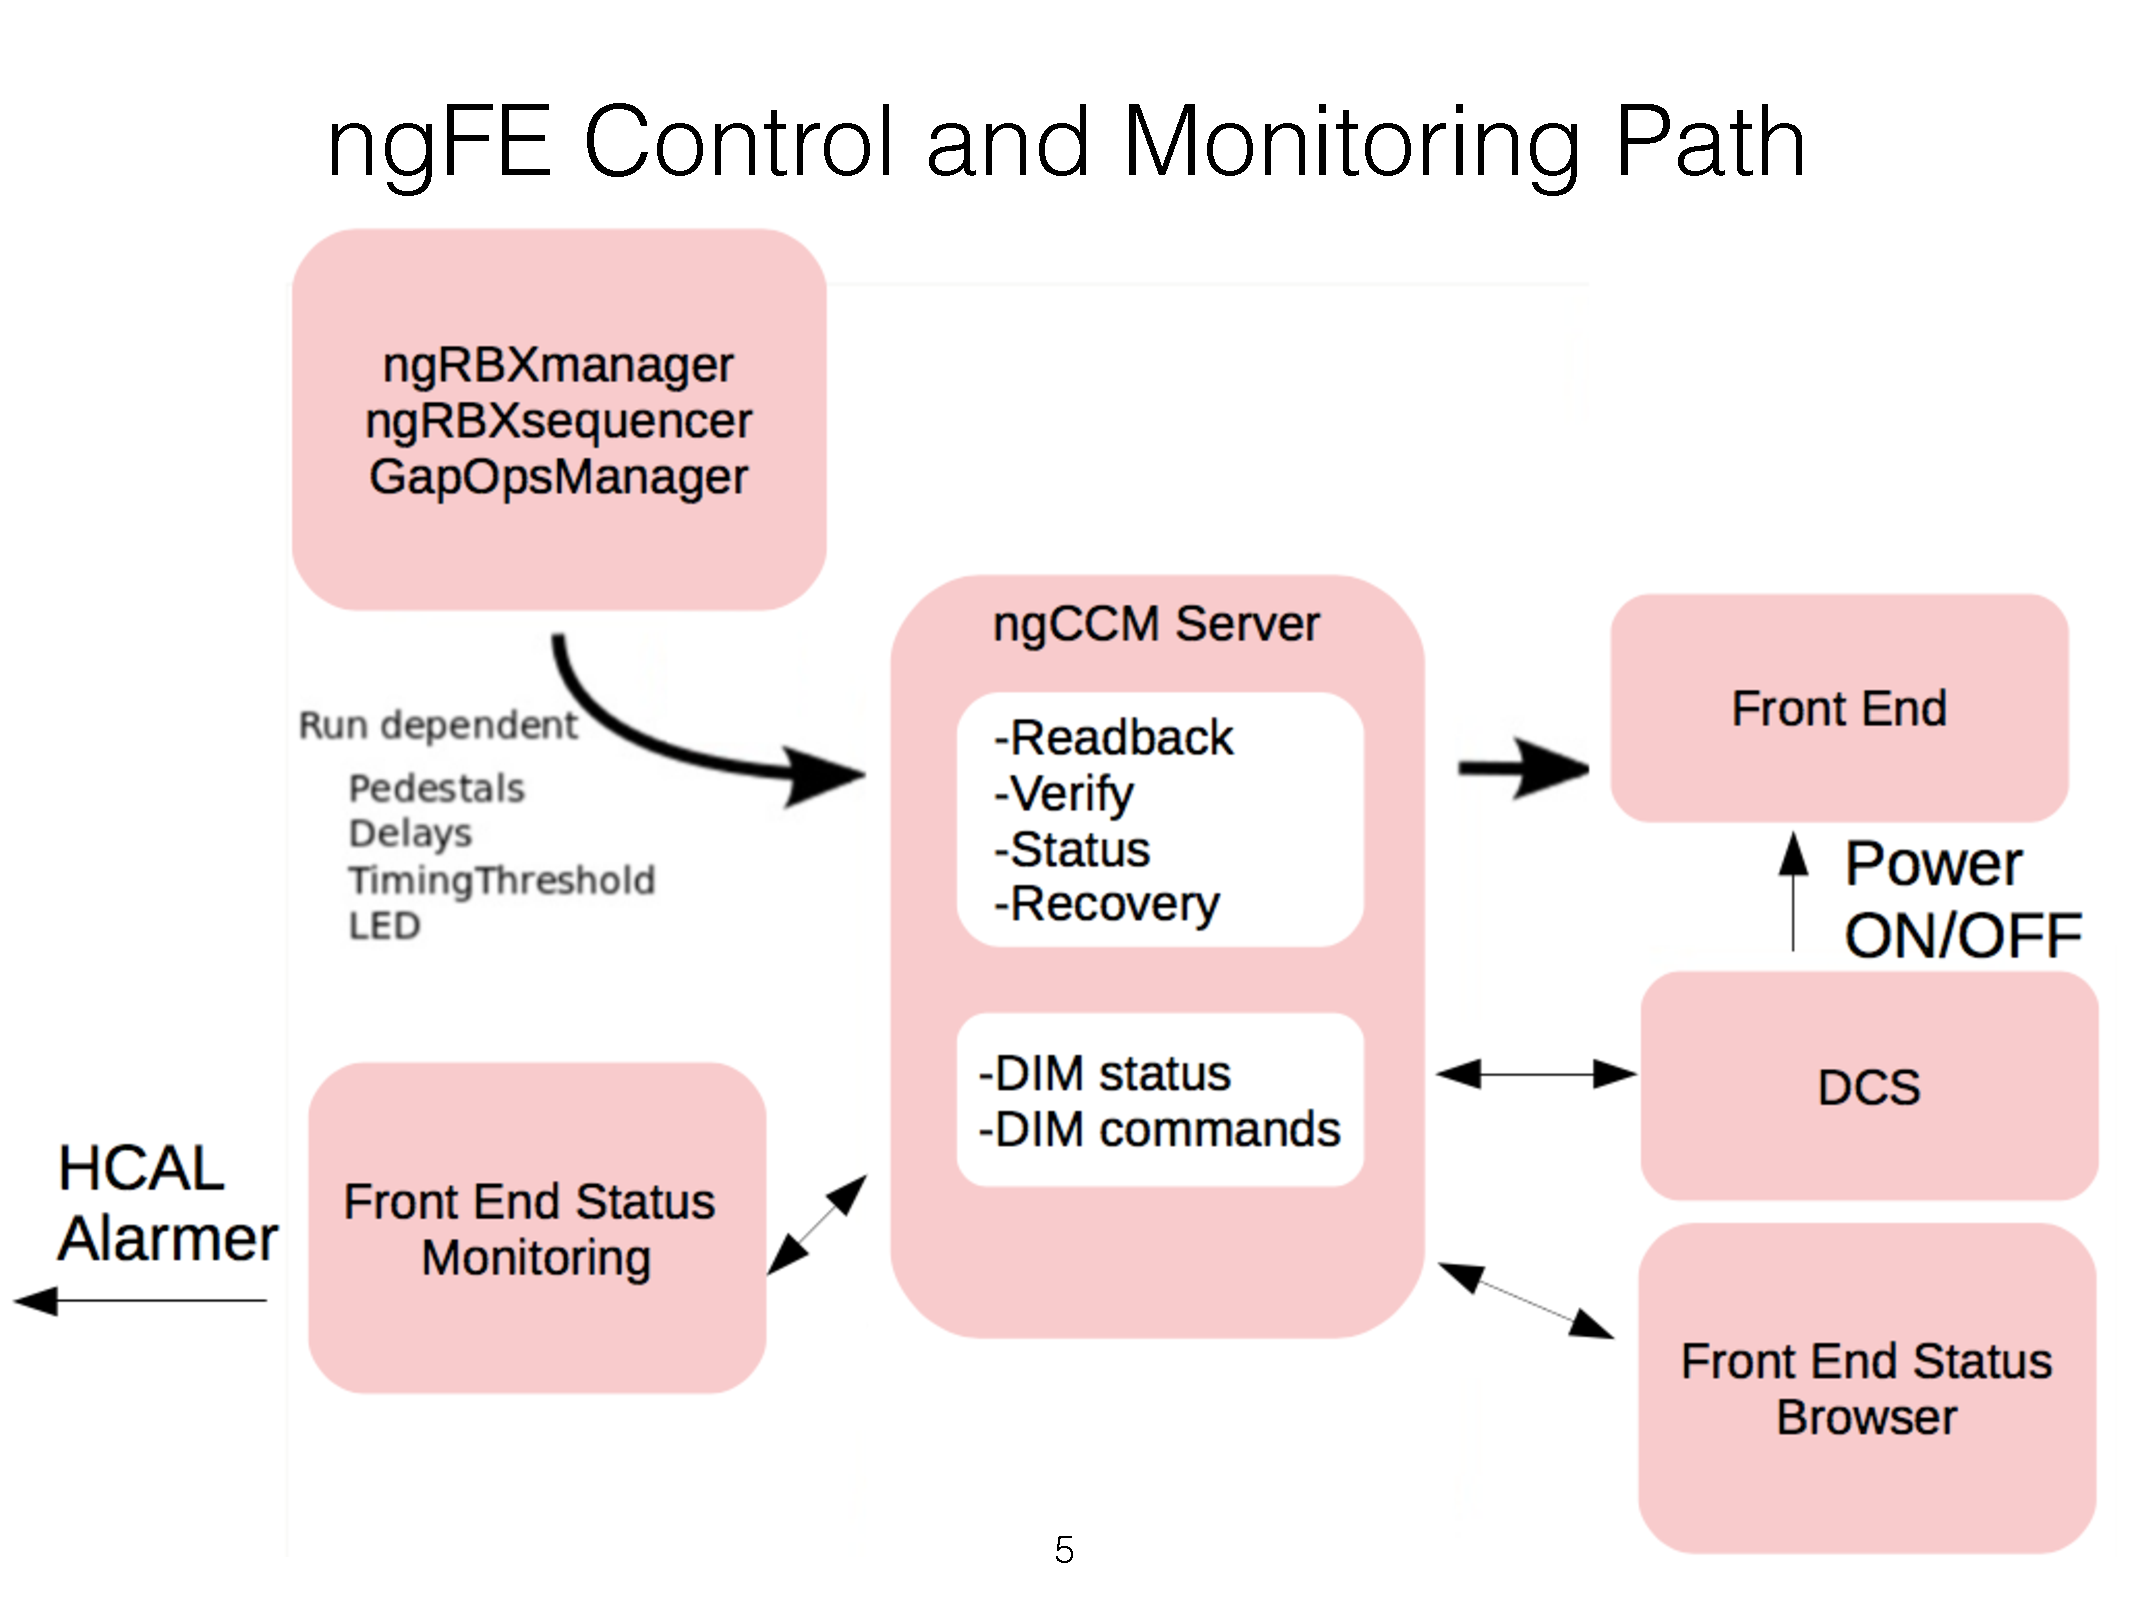
\includegraphics[width=\textwidth]{figures/ngFEsoftware.pdf}
    \caption[
        %Short caption for the list of figures
       \HCAL ngFE software control scheme. 
    ]{
        % Full caption shown below the image
       A layout of the \HCAL front-end control software for the phase I upgrade.  The ngCCM server is the central piece of software which receives communication from \HCAL applications and DCS.   
    }
    % A label so you can \ref{fig:my_fig}. It is arbitrary; neither the 'fig:'
    % nor the fact that it has the same name as the pdf are required.
    \label{fig:ngFESW}
\end{figure}

The \texttt{ngCCM server} has a unique structure, which, though complicated, has served to put several different needed software tasks into one program. The server is built with a ``devActor'' framework, where the server is made up of many individual actors, called ``guardians''. The guardians are configured when the server starts, each is responsible for a group of components of the front-end control, and any components which are ``downstream'' in communication. A guardian is created for each ngFEC the server communicates with, and a guardian for each RBX an ngFEC communicates with, these sitting under the ngFEC guardian. Commands propagate down the tree, and status information propagates up. At the base level, hardware registers have supervisors, the leaves on the tree. There are supervisors at every level with hardware registers, but majority of supervisors are for registers within RBXs. A diagram of this can be seen in Fig.~\ref{fig:ngCCMserve}
\begin{figure}[!tp]
    \centering
    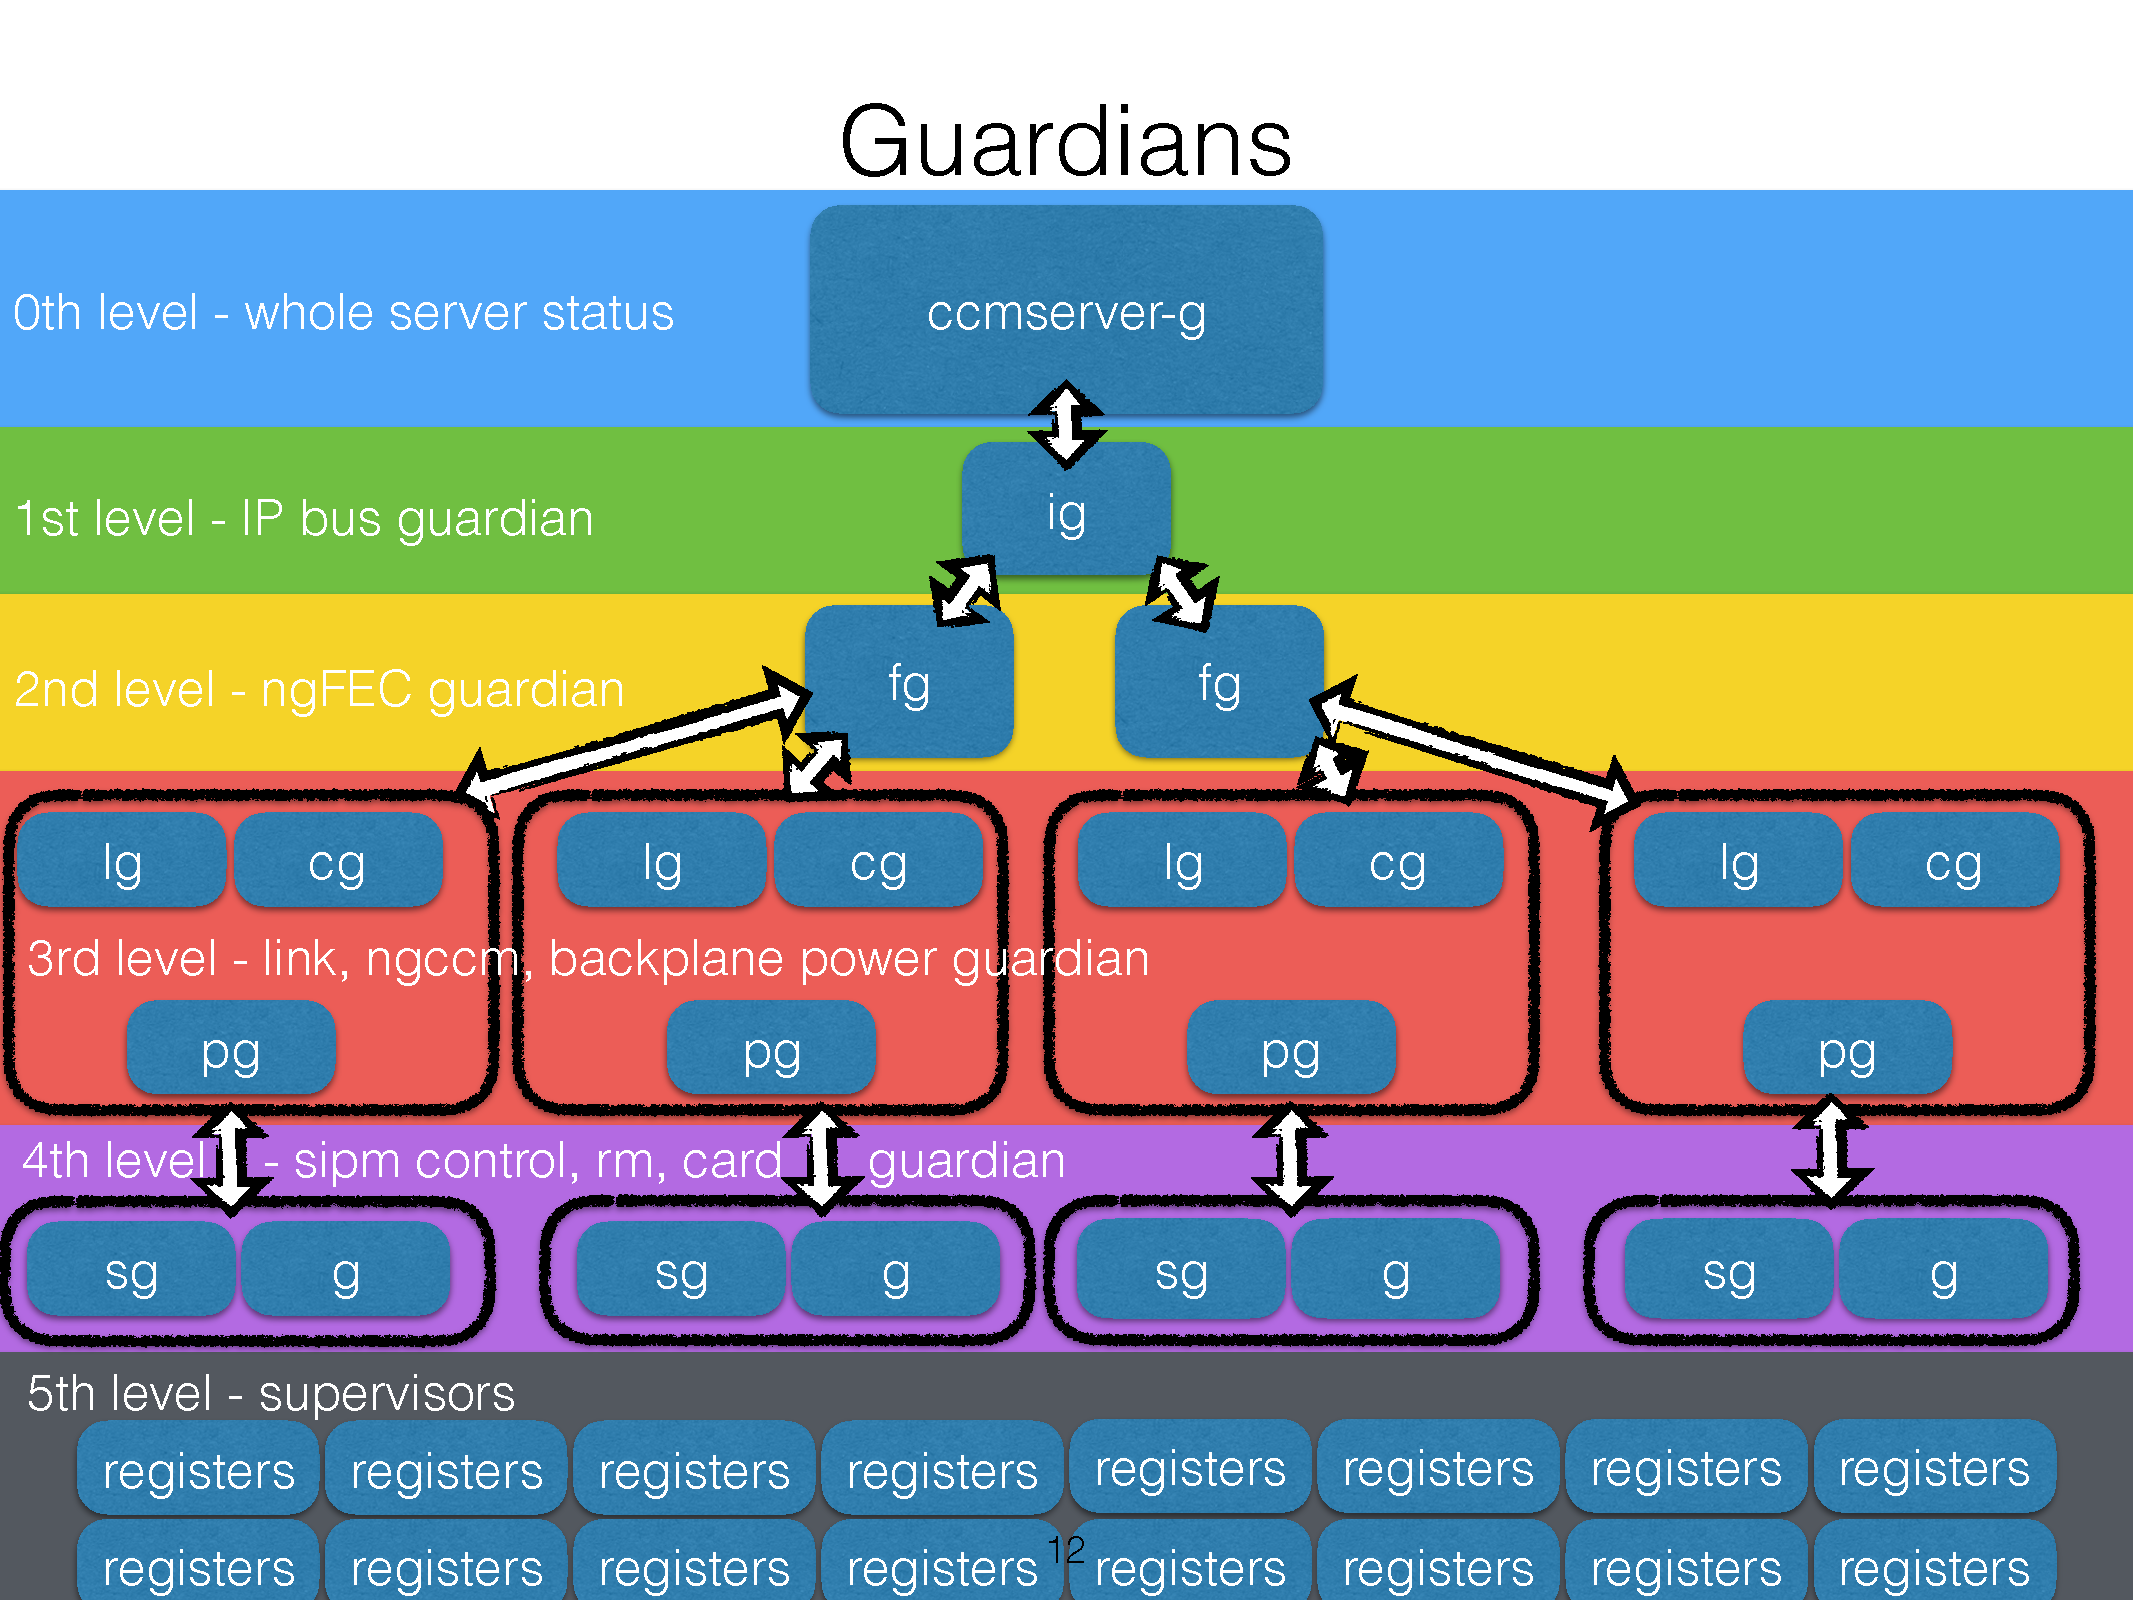
\includegraphics[width=\textwidth]{figures/ngCCMserverGuardians.pdf}
    \caption[
        %Short caption for the list of figures
       \HCAL ngCCM server guardian tree. 
    ]{
        % Full caption shown below the image
       A tree of the \texttt{ngCCM server} guardians is shown.  The trunk level being a purely software guardian for the server, this then branches out following the physical structure of the front-end system.   
    }
    % A label so you can \ref{fig:my_fig}. It is arbitrary; neither the 'fig:'
    % nor the fact that it has the same name as the pdf are required.
    \label{fig:ngCCMserve}
\end{figure}

\subsection{HEM Readout Box Failure}
On June 30th, 2018 the new endcap electronics were stress tested in an unexpected way. The smoke alarms on the surface, in the room containing the main power supplies for the cavern, triggered. The result was an almost immediate power cut to all \CMS (including \HCAL) electronics in USC. Following the power cut and recovery, two sectors on the negative \ensuremath{\eta} side of the detector (labeled HEM15 and HEM16, which make up 40 degrees of the endcap on their side) failed to power on. The power supply responsible for sending low voltage power to the control units for these sectors reported an over voltage limit error ``OvHVMax''. The power supplies responsible for each were replaced.  Power-up was successful, but communications failed. The current consumption of the readout boxes also appeared strange. Another replacement of the power supplies was attempted, and again communication was unsuccessful. A graph of the current draw of the RBXs is shown in Fig.~\ref{fig:dyingRBX}.

\begin{figure}[!tp]
    \centering
    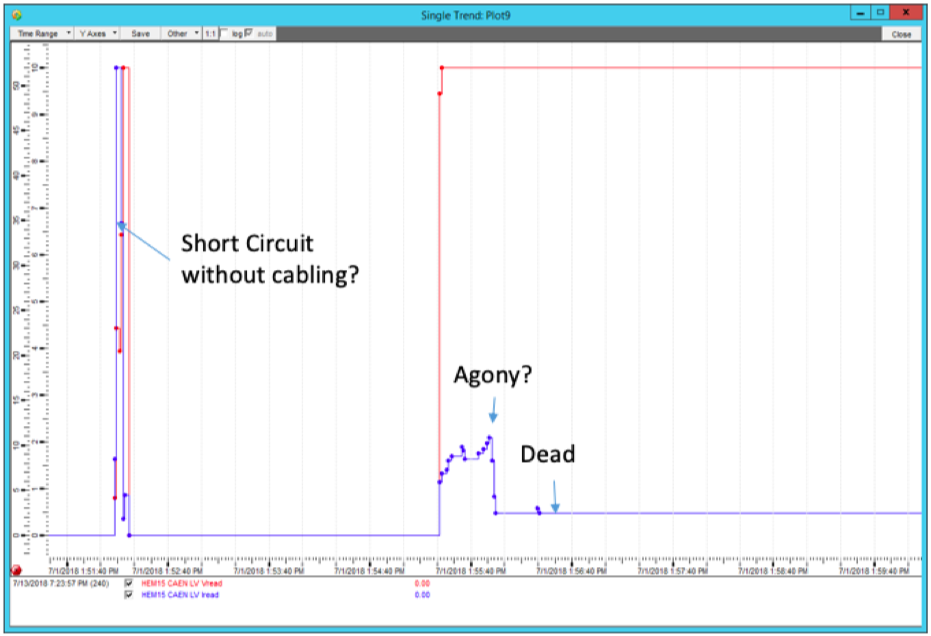
\includegraphics[width=\textwidth]{figures/DYINGRBX.png}
    \caption[
        %Short caption for the list of figures
       Failure of HEM15 RBX.
    ]{
        % Full caption shown below the image
        The voltage (red) across and current through (blue) one of the failed readout boxes, HEM15, is shown. The second jump in voltage corresponds to a current rise, fluctuation and then failure. The module was already broken at this point, and simply finishing ``frying''.  
    }
    % A label so you can \ref{fig:my_fig}. It is arbitrary; neither the 'fig:'
    % nor the fact that it has the same name as the pdf are required.
    \label{fig:dyingRBX}
\end{figure}

After extensive diagnostic tests and attempts to reproduce the event, it was determined that the power supplies had, in error, sent a voltage pulse of roughly \ensuremath{\SI{20}{V}}. Given the maximum recommended voltage of \ensuremath{\SI{12}{V}} for the module, this was sufficient to completely destroy the hardware. Due to the tight environment in which the HE RBXs are installed, it was not feasible to replace them in the middle of the 2018 data collection period. The low voltage power supplies were then taken for testing both at CERN and with the manufacturer, CAEN. After considerable testing, it was determined that under certain power-up conditions the power supply could send a brief higher voltage pulse on the low voltage line. Fearing a repeat of the issue as it was being understood, a very simple Zener diode setup was used, which would prevent the low voltage line from exceeding the Zener breakdown, allowing for a cheap and simple solution to prevent damage to the RBXs that remained functioning, but had potentially flawed power supplies. The rest of the years data was collected with HEM15 and HEM16 powered off, these make up 40 degrees of the endcap on one side.  
With 40 degrees of one endcap of \HCAL off, the physics performance of the detector is significantly affected, but not fully lost. \CMS uses information from as many sub-detectors as possible to create reconstructed "particles". Any hadronic activity entering this region then, suffers reduced precision, but is not completely lost. The amount of energy that would be expected in the dark region of \HCAL must be extrapolated. Electron identification also suffers. While there are many different properties that distinguish electrons in the detector, one key way they are distinguished from charged pions is that charged pions shower in \ECAL and \HCAL, electrons do not, as they are too light to travel this far. The ratio of energy deposited in \ECAL and \HCAL behind allows for a discrimination which is impossible with \HCAL off. The specific effects on this analysis was studied and is discussed later in section \ref{sec:HEMfailure}.




%%%%%%%%%%%%%%%%%%%%%%%%%%%%%%%%%%%%%%%%%%%%%%%%%%%%%%%%%%%%%%%%%%%%%%%%%%%%%%%%
